\documentclass{article}
\usepackage[utf8]{inputenc}
\usepackage{amsmath}
\usepackage{graphicx}
\usepackage{hyperref}
\usepackage[english]{babel}\usepackage{subcaption}
\usepackage{sidecap}
\usepackage{lipsum}
\usepackage{multicol}
\usepackage{sectsty}
\usepackage{caption}
\usepackage{placeins}
\usepackage{subcaption}
\usepackage{bm}
\usepackage[dvipsnames]{xcolor}

\definecolor{myred}{RGB}{143, 42, 12}
\definecolor{myblue}{RGB}{58, 83, 197}
\definecolor{myorange}{RGB}{219, 146, 0}
\newcommand{\centered}[1]{\begin{tabular}{l} #1 \end{tabular}}

% \sectionfont{\centering}
\usepackage[a4paper,top=2cm,bottom=2cm,left=2cm,right=2cm]{geometry}
\title{\textbf{Robotics II} \\ \large{\textbf{Final Project}}}
\author{Marco Pennese 1749223, Veronica Vulcano 1760405}
\date{}

\begin{document}
\maketitle
\tableofcontents
\pagebreak

\section{Introduction}
\paragraph{}The goal of our work is to perform the dynamic identification of a robot, estimating its dynamic parameters/coefficients by solving an optimization problem. As we know, it is very important to have an accurate dynamic model because it allows us to implement better control laws for achieving many tasks.
\paragraph{}In particular, we have dealt with the problem of torque sign lack, as it happens in some real robot (e.g., KUKA KR5). In fact, when we know only the absolute value of torque and we do not have the knowledge about the torque sign, we cannot use traditional methods for dynamic identification. For this reason, we have developed an algorithm able to estimate torque signs so that we could proceed with the identification using well known strategies.
\paragraph{}In our work, we first studied a simple 1R robot under gravity; then, we moved to a more complex robot, a 3R spatial robot. For both of them, we are now reporting the procedure we followed, the simulations and the results of our experiments.\\

The repository of our work is available here \url{https://github.com/MarcoPenne/Robotics_Project}.

\section{1R arm under gravity}
\paragraph{}We start our work by focusing on a simple robot arm (pendulum) under gravity.
\subsection{Dynamic model}
\paragraph{} 
The dynamic model of this kind of robots is:
\[\tau=gmd \sin(q) + (I+md^2)\ddot{q}= \begin{bmatrix}
\sin(q) & \ddot{q}
\end{bmatrix}\begin{bmatrix}
gmd \\ I +md^2
\end{bmatrix}\]
where $\tau$ are the joint torques, $m$ is the mass of the link, $I$ is the moment of inertia, $d$ is the position of the center of mass with respect to the rotating axis and $g$ is the gravitational acceleration.

\begin{figure}[!htbp]
\centering
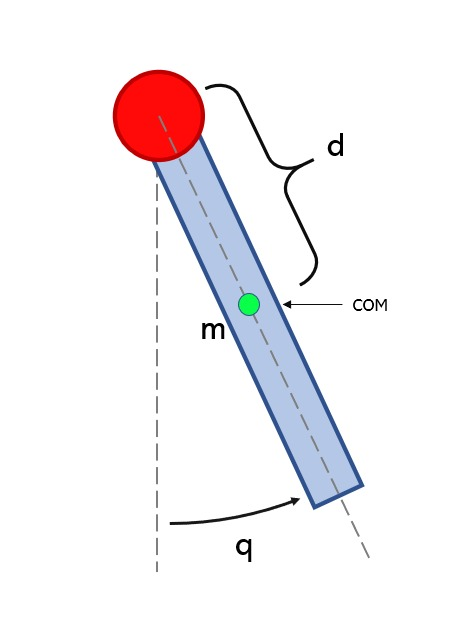
\includegraphics[width=0.3\textwidth]{images/1-dof/model.jpeg}
\caption{Robot arm model: $m$ is the mass of the link, $d$ is the position of the center of mass, $I$ is the moment of inertia when rotating around the center of mass}
\end{figure}
\FloatBarrier

\paragraph{} We generate some trajectories from which we can compute the torques and build the $Y$ matrix for a certain time instant. Then, we stack all the $Y$ in a unique matrix $\overline{Y}$ (regressor matrix) and we do the same also for the measured torques obtaining a vector $\overline{\tau}$. \\\\
$\overline{Y}$ and $\overline{\tau}$ are the inputs of the PBPR algorithm.

\subsection{PBPR algorithm}
\paragraph{}Given a robot, we have a number of dynamic parameters to consider (mass, inertia tensor and center of mass); the robot dynamics depends in a nonlinear way on some of these parameters. It is possible to reorganize the dynamic parameters so that they appear only in a linear fashion; by doing some computations, we can obtain a minimum number of terms that we call dynamic coefficients of the robot $\pi$ and they are the only ones that appear in the model, so the only ones we need to know. Having a minimum number of parameters is advantageous because when we do experiments for identifying these terms, it  will give a more reliable identification (we are not spreading data on a number of parameters that are dependent one to the other).

\paragraph{}The aim of the Penalty-Based Parameters Retrieval (PBPR) algorithm is to get a physically consistent set of dynamic parameters; in order to do so, we need to solve the following optimization problem:
\[\min_{p_k}{\phi(p_k)} = \lVert \overline{Y}\pi(p_k)-\overline{\tau} \rVert^2\]

\noindent where $\overline{Y}$ is the stacked regressor, $\overline{\tau}$ is the stacked  torque measurements and $\pi(p_k)$ is the coefficients vector computed from the current parameters vector $p_k$.

\paragraph{}In order to obtain a physically consistent set of parameters, we should put constraints on the mass and on the inertia. Since we are dealing with a 1-dof robot, the only constraint we have is that both mass and inertia should be positive:

\[m > 0, I > 0\]

In general, it is possible to provide a set of lower and upper bounds for the dynamic parameters based on a priori knowledge. For instance, the center of mass must be inside the convex link of the robot. 

\paragraph{}However, we cannot apply directly this algorithm to our context because we do not have torque signs.  We need a preliminary analysis in which we predict what are the most likely torque signs.

\subsection{Tree of solutions}
\paragraph{}First of all, we take the absolute values of the generated torques so to pretend that we have not this kind of information. The idea behind the implementation of the algorithm is the following.\\

We can imagine that neighboring torques have the same sign. So, we have that subsequent torque values usually have the same sign, then the absolute value starts to decrease approaching zero, until it crosses zero and possibly changes sign. As a consequence, we have to "mark" the function whenever it crosses 0. In order to do this, we should tolerate a threshold; we compute this threshold by discarding the 10\% of samples closer to 0. At this point, we discard all the samples under threshold; we are left with several segments (i.e.,  sequences of points) so that in each of them the sign of the torque is either positive or negative.

\paragraph{}We can evaluate the regression matrix $Y$ at each instant of time:

\vspace{1em}
\[\begin{bmatrix}
Y(q(t_1),\dot{q}(t_1),\ddot{q}(t_1))\\
\vdots \\
Y(q(t_n),\dot{q}(t_n),\ddot{q}(t_n))
\end{bmatrix} \begin{bmatrix}
gmd \\ I +md^2
\end{bmatrix} = \begin{bmatrix}
\tau(t_1)\\
\vdots \\
\tau(t_n)
\end{bmatrix} \]
\vspace{1em}

Notice that the sign of the regression matrix is certain, because $Y$ depends on the values of position, velocity and acceleration. From this formula, we infer that it is possible to treat all the segments one indipendently from the other, because each torque at a given time instant has its own $Y$'s row. We can rewrite the previous formula so as it fits our problem (in the case of $n$ segments):

\vspace{1em}
\[\begin{bmatrix}
Y_{seg_1}(t_{i_1}, ..., t_{f_1})\\
\vdots \\
Y_{seg_n}(t_{i_n}, ..., t_{f_n})
\end{bmatrix} \begin{bmatrix}
gmd \\ I +md^2
\end{bmatrix} = \begin{bmatrix}
\tau_{seg_1}(t_{i_1}, ..., t_{f_1})\\
\vdots \\
\tau_{seg_n}(t_{i_n}, ..., t_{f_n})
\end{bmatrix} \]
\vspace{1em}

While dealing with a single segment, we take the corresponding $Y$ and $\tau$  blocks. So, for the $k^{th}$ segment the problem becomes:

\[Y_{seg_k}(t_{i_k}, ..., t_{f_k})
\begin{bmatrix}
gmd \\ I +md^2
\end{bmatrix} =
\tau_{seg_k}(t_{i_k}, ..., t_{f_k})\]

By taking the segments independently, it may be the case in which $Y_{seg_k}$ has not full rank. So, we need something to deal with this possibility and always have well defined problems. To compute the order in which the segments will be considered, we choose as heuristic function  the one that computes the condition number of $Y_{seg_k}$. In fact, a problem with a high condition number is said to be ill-conditioned; this means that the solution to the problem is difficult to find. We can define a threshold for the condition number; if the condition number of all $Y_{seg_k}$ is over this threshold, we start considering all the possible pairs $(Y_{seg_j},Y_{seg_k})$; if we are still over-threshold, then we consider groups of three $(Y_{seg_i},Y_{seg_j},Y_{seg_k})$, then four and so on. At this stage, we have a well defined problem from which we can start predicting the torque signs; any problem with fewer segments would not be as good as the one we have.

\paragraph{}After that, we have to predict the torque sign for each segment. The previous step returns the order in which segments should be considered so as the condition number decreases. The idea is: we take the first segment which could be either positive or negative, so we have two possible solutions; then, we take the following segment in the sequence which again could be either positive or negative, so at this stage we have four possible solutions (by considering the previous ones), and so on. This is an exponential problem, so if we have $n$ segments we would have $2^n$ possible solutions. However, it is possible to prevent the tree from being completely expanded because we can recognize in advance when a choice of sign lead to a wrong solution; in fact, when the PBPR algorithm is applied to a torque with the wrong sign, the loss should be higher than the one with the correct sign. So, at each level of the tree, we expand only the best nodes which are the ones with the lowest loss among the segments at disposal (in our case, we decided to expand the best 5 nodes).  It could happen that by expanding only few nodes per level we cut some potentially good branch; we need this tradeoff to improve the computational time and therefore the performance of the algorithm. In any case, we will notice about this at the end. For all the optimization problems of the tree we use pattern search algorithm because it is faster.

\paragraph{}At the end of this tree algorithm, we will obtain the best combination of signs for the segments sequence. So, we apply the PBPR algorithm to this sequence with a number of runs equal to 3 using simulated annealing.\\

In this section, we had only one joint to consider; we will see how segments are handled in the case of multiple joints further on.

\subsection{Experiments}
\paragraph{Experiment 1}
For our experiments, we start with a very simple trajectory in which the initial configuration of the robot robot is $q = 0$, then it goes to the configuration $q = \dfrac{\pi}{4}$ and finally it returns to the initial configuration. In order to obtain such trajectory, we interpolate these points with a cubic spline. With this trajectory, the resulting torques are always positive, so it will be easier for the algorithm to compute the sign.

\begin{figure}[!htbp]
\centering
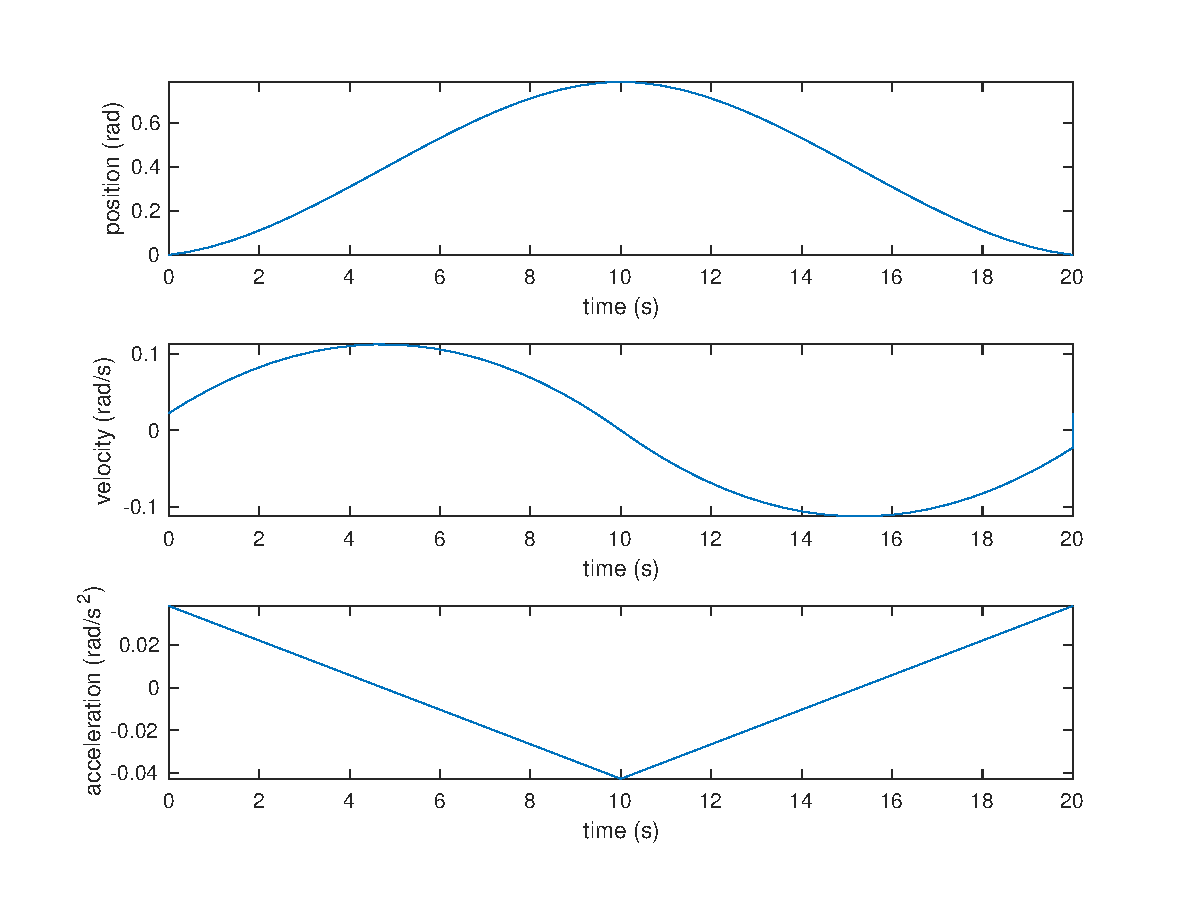
\includegraphics[width=0.7\textwidth]{images/1-dof/trajectory_easy1.eps}
\caption{Plot of position, velocity and acceleration; the last two are obtained by symbolic differentiation}
\end{figure}
\FloatBarrier

From these values, we obtain the torques by computing the $Y$ matrix, the dynamic coefficients $\pi$ and multiplying them. The dynamic parameters are up to our choice, so we invented their values in order to compute the dynamic coefficients. \\

At this point, we stack all the $Y$ and $\tau$ together. Then, we take the absolute values of $\tau$ and send them to the tree algorithm. Finally, we send $\overline{Y}$ and $\overline{\tau}$ with the estimated signs to the PBRP algorithm. \\

We report the results:

\begin{table}[!htbp]
\centering
\begin{tabular}{|c|cc|}
\hline
& Ground truth & Retrieved\\
\hline
$m\;[kg]$ & 5 & 5.8590\\ 
$d\;[m]$ & 0.5 & 0.4267\\
$I\;[kg\cdot m^2]$ & 0.4208 & 0.6041\\
\hline
\end{tabular}
\caption{Dynamic parameters}
\end{table}
\FloatBarrier

We remember that:

\[\bm{\pi}= \begin{bmatrix}
\pi_1 \\ \pi_2
\end{bmatrix} = \begin{bmatrix}
gmd \\ I +md^2
\end{bmatrix}= \begin{bmatrix}
24.5250 \\ 1.6709
\end{bmatrix}\]

The estimated dynamic coefficients are:

\[\bm{\hat{\pi}}= \begin{bmatrix}
\hat{\pi}_1 \\\hat{ \pi}_2
\end{bmatrix} =
\begin{bmatrix}
24.5250 \\ 1.6709
\end{bmatrix}\]

Even if there is a slightly difference between the ground dynamic parameters and the estimated ones, we obtain the same dynamic coefficients. As a measure of the error, we take the norm of the difference between the ground values of the dynamic coefficients and the estimated ones; in this experiment, we obtain an error equal to $1.6410\cdot10^{-5}$.

\begin{figure}[!htbp]
\centering
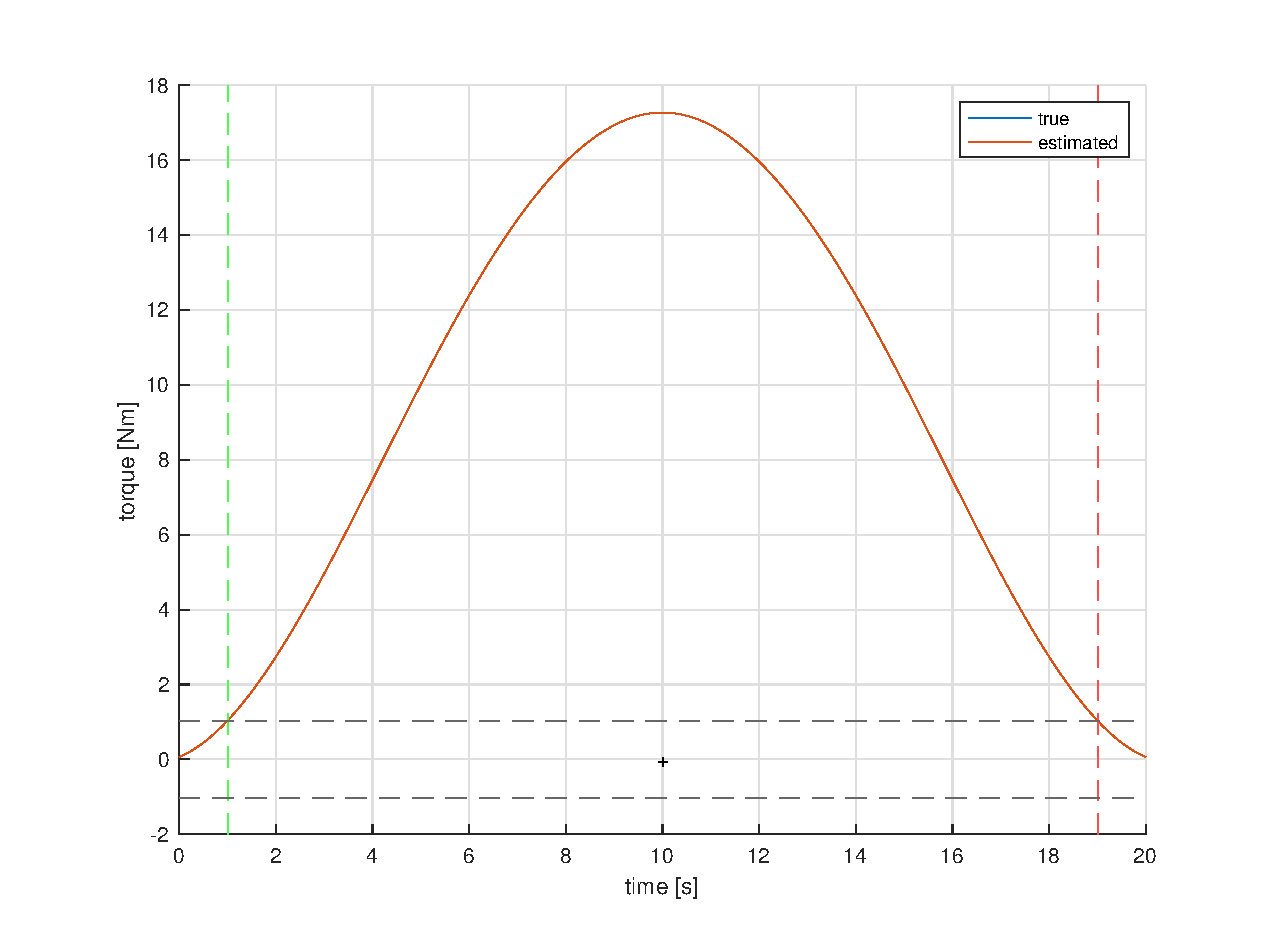
\includegraphics[width=0.7\textwidth]{images/1-dof/results1.eps}
\caption{Plot of the reconstructed torque vs nominal torque. The gray dashed lines represent the threshold; the green dashed lines represent the start of the segment, while the red dashed lines represent the end of the segment. Samples under threshold are discarded. The signs estimated by the algorithm are reported for each segment.}
\end{figure}
\FloatBarrier

\paragraph{Experiment 2}Then, we move to a slightly more difficult trajectory, in which the robot starts from $q = 0$, then it goes to the configuration $q = \dfrac{\pi}{4}$, then to $q = -\dfrac{\pi}{4}$ and finally it returns to the initial configuration. Again, we interpolate these points with a cubic spline. With this trajectory, the resulting torques are positive in the first half period and negative in the second one.

\begin{figure}[!htbp]
\centering
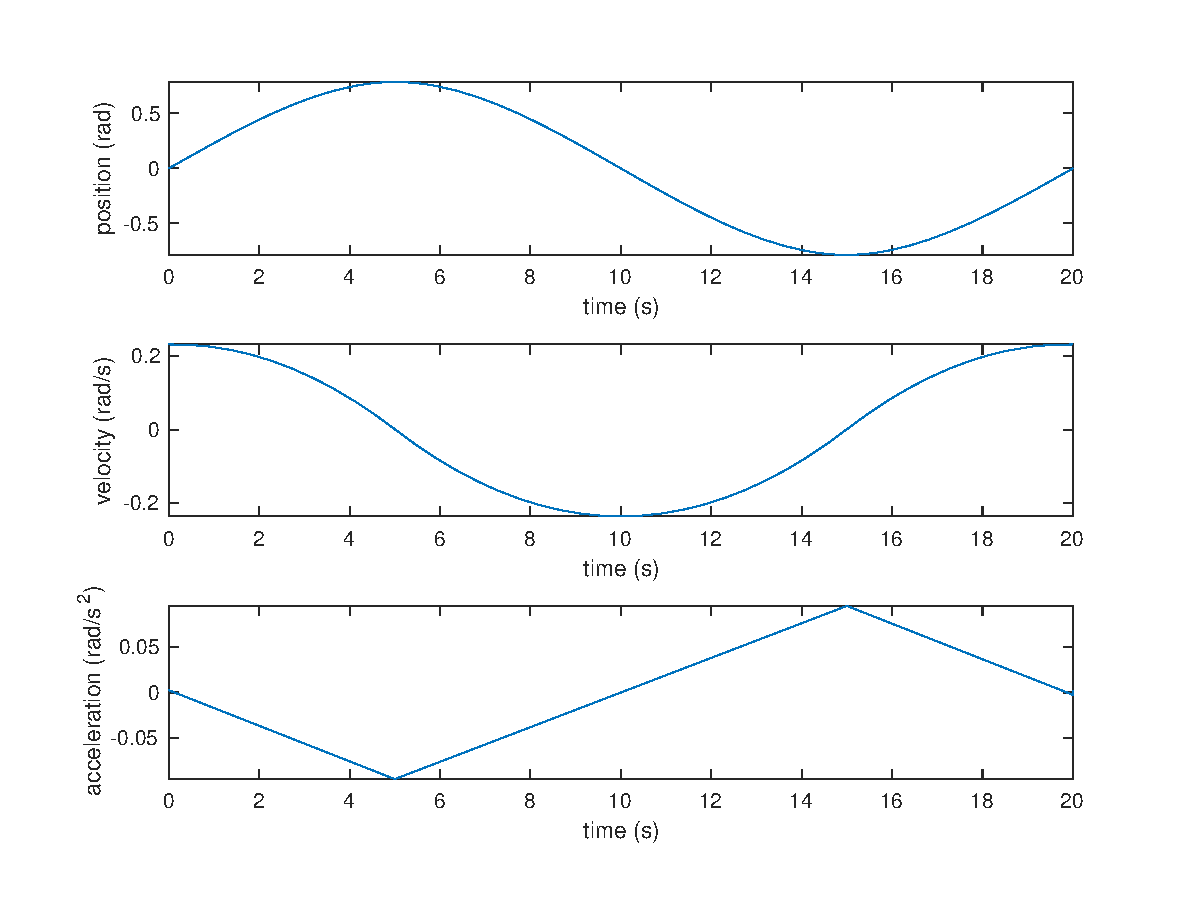
\includegraphics[width=0.7\textwidth]{images/1-dof/trajectory_easy2.eps}
\caption{Plot of position, velocity and acceleration; the last two are obtained by symbolic differentiation}
\end{figure}
\FloatBarrier

We follow the same procedure as before and we obtain:

\begin{table}[!htbp]
\centering
\begin{tabular}{|c|cc|}
\hline
& Ground truth & Retrieved\\
\hline
$m\;[kg]$ & 5 & 6.3695\\ 
$d\;[m]$ & 0.5 & 0.3926\\
$I\;[kg\cdot m^2]$ & 0.4208 & 0.7316\\
\hline
\end{tabular}
\caption{Dynamic parameters}
\end{table}
\FloatBarrier

The estimated dynamic coefficients are:

\[\bm{\hat{\pi}}= \begin{bmatrix}
\hat{\pi}_1 \\\hat{ \pi}_2
\end{bmatrix} =
\begin{bmatrix}
24.5295 \\ 1.7132
\end{bmatrix}\]

In this case, we do not obtain the exactly same values of the dynamic coefficients; this is reflected in the value of the error, which is larger than before ($4.2554 \cdot 10^{-2}$).

\begin{figure}[!htbp]
\centering
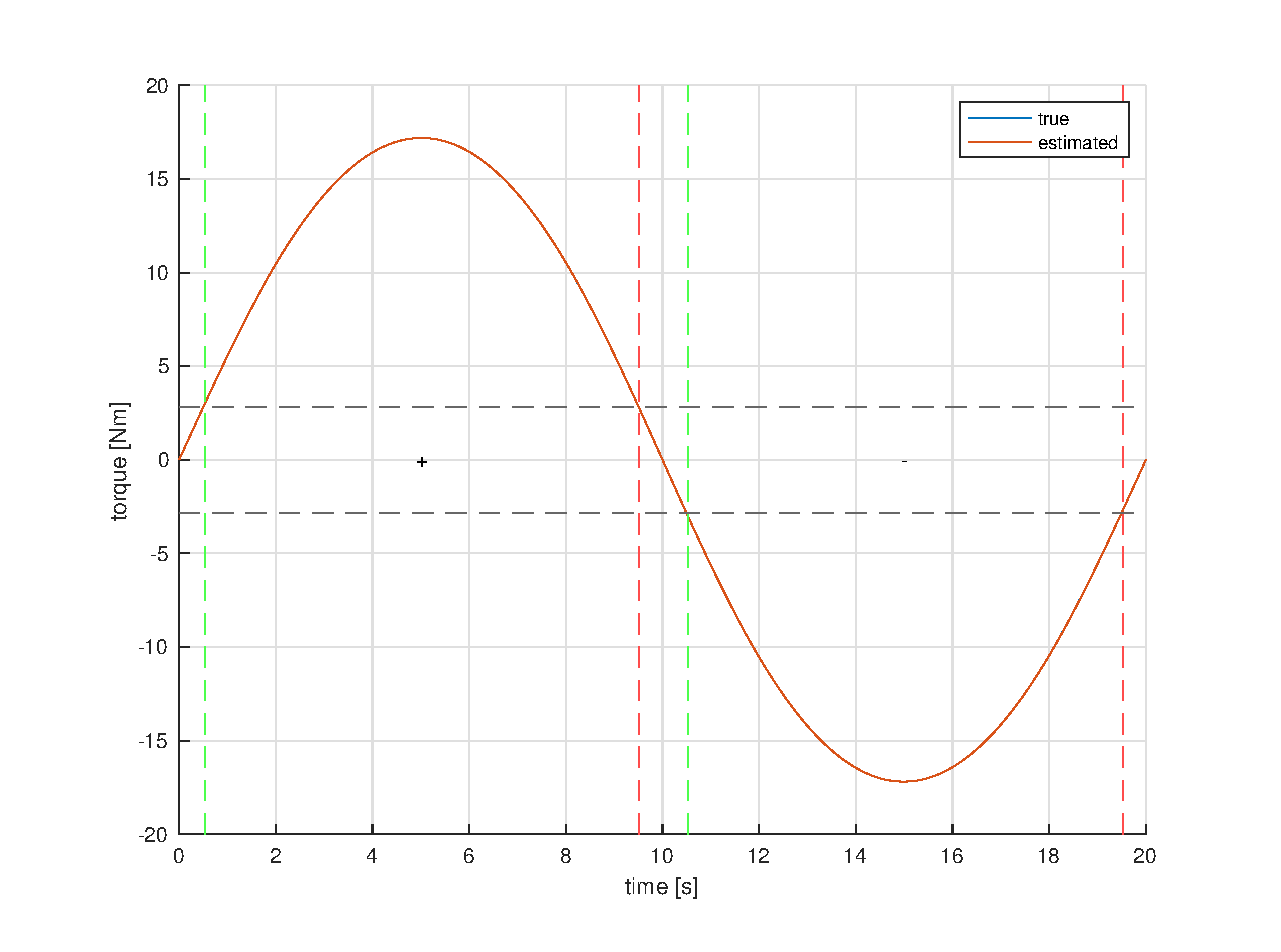
\includegraphics[width=0.7\textwidth]{images/1-dof/results2.eps}
\caption{Plot of the reconstructed torque vs nominal torque. The gray dashed lines represent the threshold; the green dashed lines represent the start of the segment, while the red dashed lines represent the end of the segment. Samples under threshold are discarded. The signs estimated by the algorithm are reported for each segment.}
\end{figure}
\FloatBarrier

\paragraph{Experiment 3} In the last experiment for the 1-dof arm, we moved to a more exciting trajectory generated according to this formula:
\[q_j(t) = \sum_{l=1}^{L}{\frac{ a_{l,j}}{ l\omega_f }\sin(l\omega_f t)-\frac{ b_{l,j}}{l\omega_f}\cos(l\omega_f t)+q_{0,j}}\]
We implemented a function called generate\_exciting\_traj() that generates a random exciting trajectory using the following parameters: $L = 5$ and $\omega_f = 0.2\pi$.

\begin{figure}[!htbp]
\centering
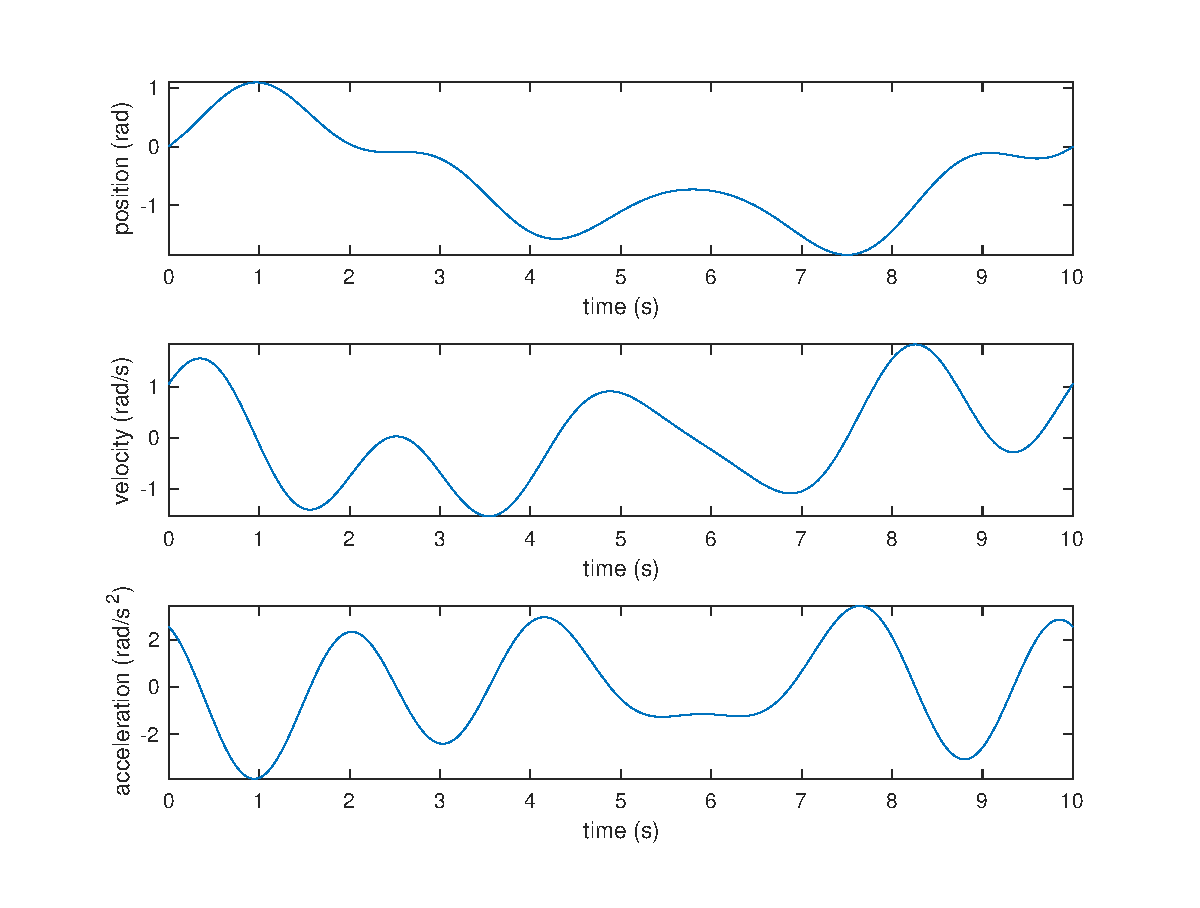
\includegraphics[width=0.7\textwidth]{images/1-dof/trajectory1.eps}
\caption{Plot of position, velocity and acceleration; the last two are obtained by symbolic differentiation}
\end{figure}
\FloatBarrier

We follow the same procedure as before and we obtain:

\begin{table}[!htbp]
\centering
\begin{tabular}{|c|cc|}
\hline
& Ground truth & Retrieved\\
\hline
$m\;[kg]$ & 5 & 7.5379\\ 
$d\;[m]$ & 0.5 & 0.3317\\
$I\;[kg\cdot m^2]$ & 0.4208 & 0.8417\\
\hline
\end{tabular}
\caption{Dynamic parameters}
\end{table}
\FloatBarrier

The estimated dynamic coefficients are:

\[\bm{\hat{\pi}}= \begin{bmatrix}
\hat{\pi}_1 \\\hat{ \pi}_2
\end{bmatrix} =
\begin{bmatrix}
24.5250 \\ 1.6708
\end{bmatrix}\]

With this experiment, we obtain almost the same dynamics coefficients; the error we get, which is equal to $2.0259\cdot10^{-6}$, is the smallest among all the experiments.  The fact that the error is smaller than the previous cases means that the system has been excited appropriately.

\begin{figure}[!htbp]
\centering
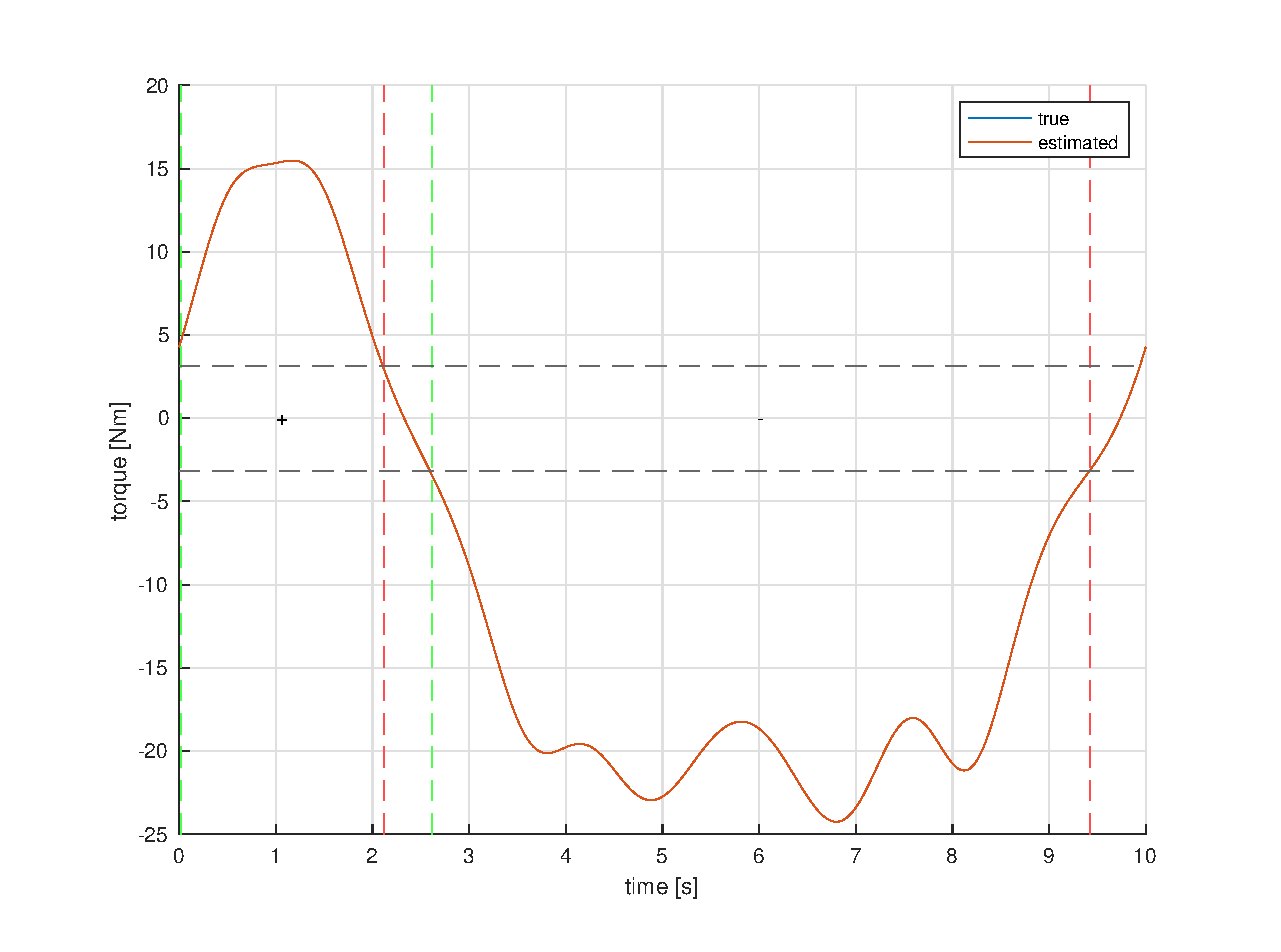
\includegraphics[width=0.7\textwidth]{images/1-dof/results3.eps}
\caption{Plot of the reconstructed torque vs nominal torque. The gray dashed lines represent the threshold; the green dashed lines represent the start of the segment, while the red dashed lines represent the end of the segment. Samples under threshold are discarded. The signs estimated by the algorithm are reported for each segment.}
\end{figure}
\FloatBarrier

\pagebreak

\subsection{Validation} \paragraph{} We validate the results obtained in the third experiment on a new never seen trajectory:

\begin{figure}[!htbp]
\centering
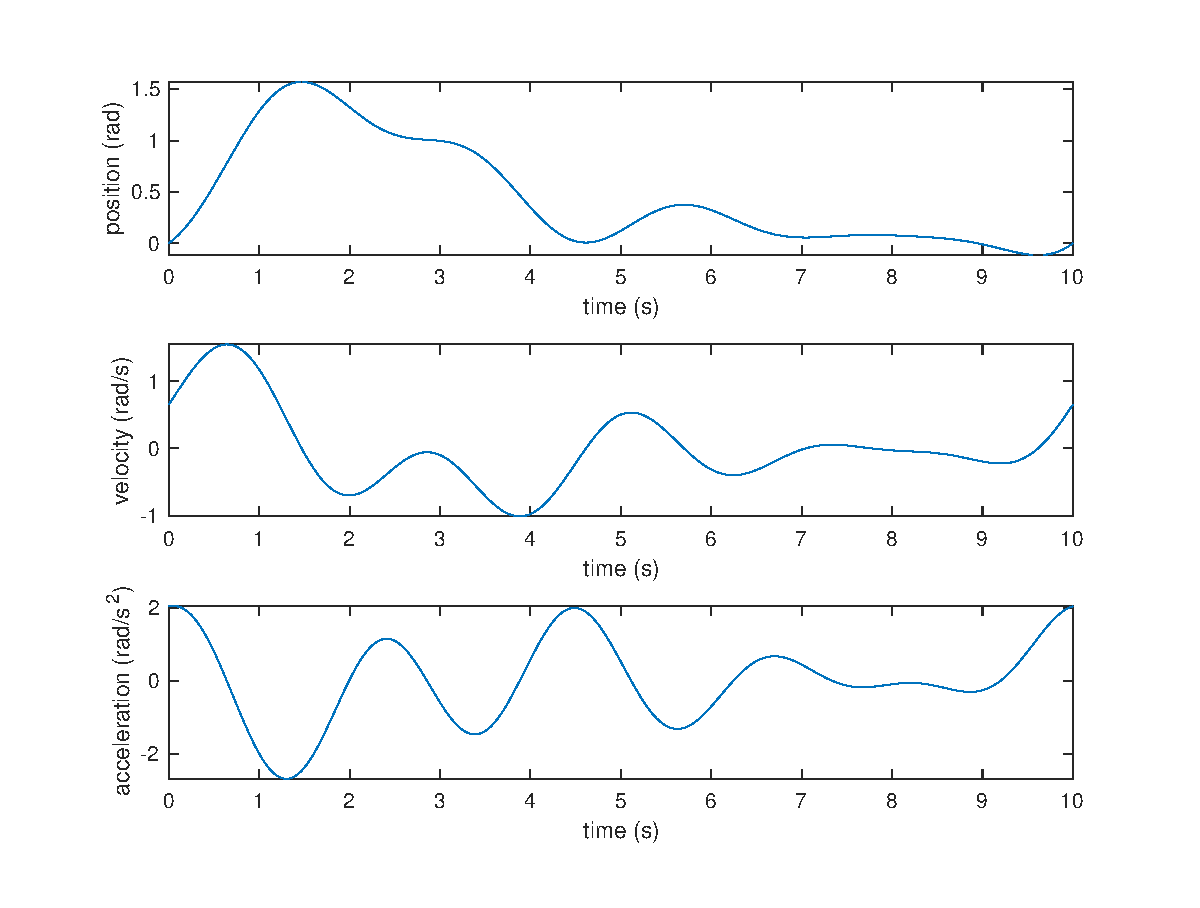
\includegraphics[width=0.7\textwidth]{images/1-dof/validation_trajectory.eps}
\caption{Plot of position, velocity and acceleration; the last two are obtained by symbolic differentiation}
\end{figure}
\FloatBarrier

The predicted torques are:

\begin{figure}[!htbp]
\centering
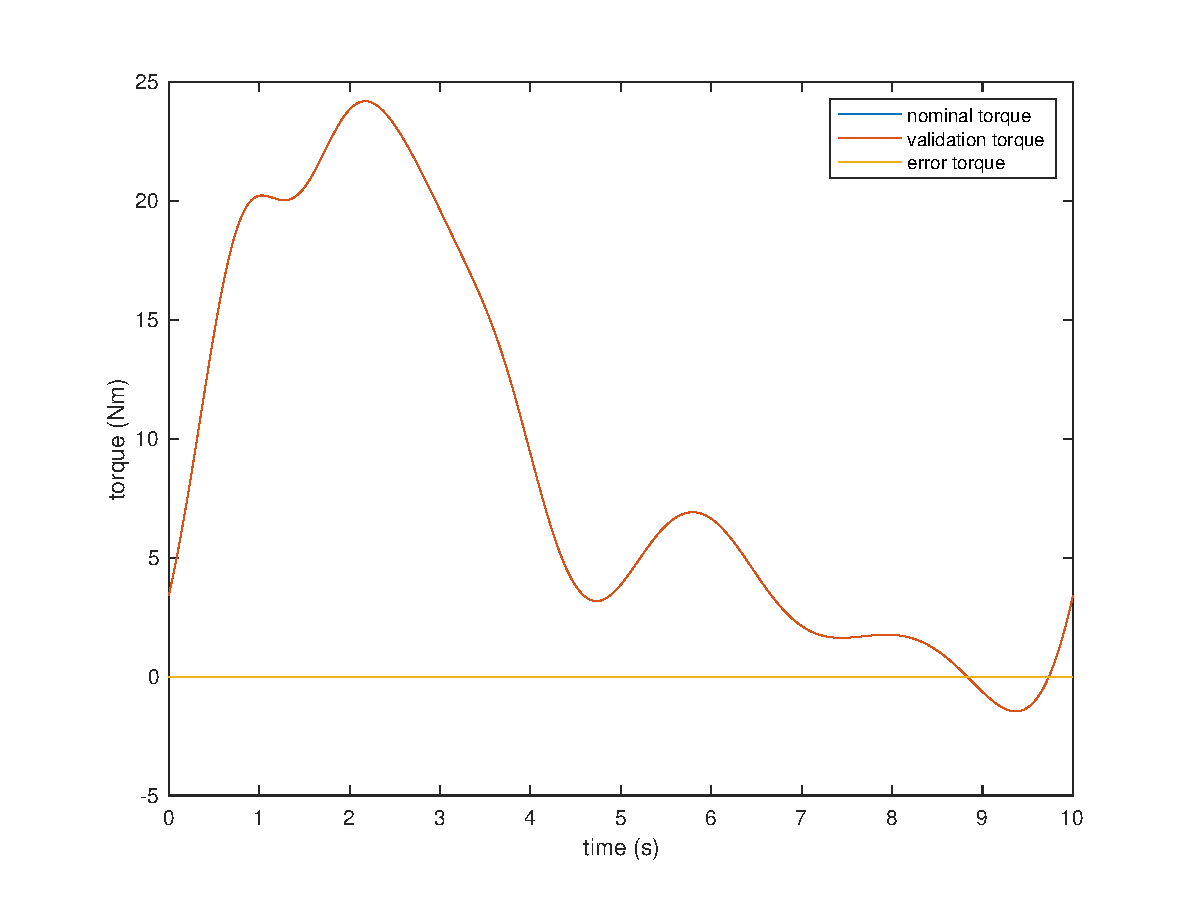
\includegraphics[width=0.7\textwidth]{images/1-dof/validation.eps}
\caption{Plot of the nominal torque vs validation torque; the error is computed as nominal torque - validation torque}
\end{figure}
\FloatBarrier

\pagebreak

\section{3R spatial robot}
After the simple case, we tried to extend this procedure to a more complex robot: a 3R spatial robot.\\
So, first of all we needed to determine the structure of the robot by defining the Denavit-Hartenberg parameters and to determine the symbolic dynamic model of the robot.
\subsection{Robot structure}
\subsubsection*{Denavit-Hartenberg}
\paragraph{}
\FloatBarrier
\begin{table}[!htbp]
\centering
\begin{tabular}{|c|cccc|}
\hline
& $\alpha$ & a & d & $\theta$\\
\hline
link 1 & $\pi$/2 & 0 & $L_1=0.3$ & $q_1$\\
link 2 & 0 & $L_2=0.3$ & $-d_2=-0.09$ & $q_2$\\
link 3 & 0 & $L_3=0.2$ & 0 & $q_3$\\
\hline
\end{tabular}
\caption{In this table the DH parameters of the robot are reported.}
\end{table}
\subsubsection*{D-H Frames}

\begin{center}
\begin{figure}[!htb]
   \begin{minipage}{0.33\textwidth}
     \centering
     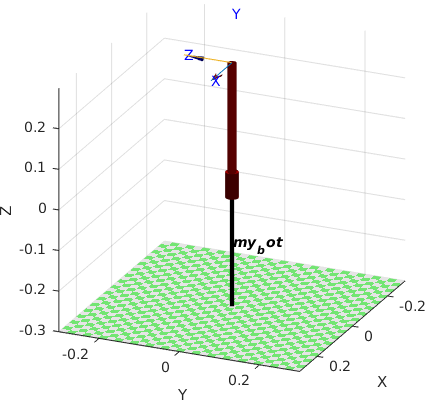
\includegraphics[width=\linewidth]{images/3-dof/frame1.png}
   \end{minipage}\hfill
   \begin{minipage}{0.33\textwidth}
     \centering
     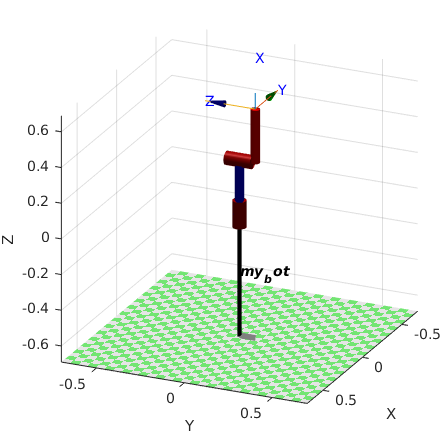
\includegraphics[width=\linewidth]{images/3-dof/frame2_q2_90.png}
   \end{minipage}\hfill
   \begin{minipage}{0.33\textwidth}
     \centering
     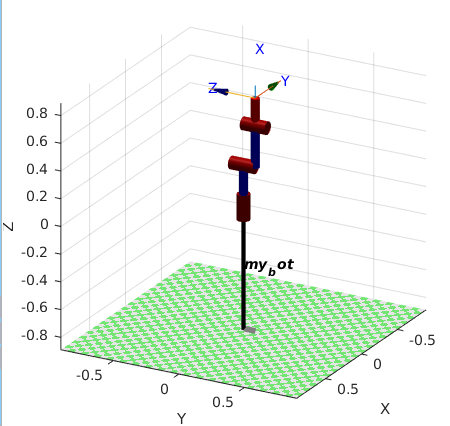
\includegraphics[width=\linewidth]{images/3-dof/frame3_q2_90.png}
   \end{minipage}
   \caption{(a) Frame 1 (b) Frame 2 (c) Frame 3}

\end{figure} 
\end{center}
\FloatBarrier

\subsubsection*{Centers of Mass}
We computed the position of the centers of mass in their respective frames, according to the DH frames we just defined.

\[r_{c1}=\begin{pmatrix}
0\\
-a\\
0\\
\end{pmatrix} = \begin{pmatrix}
0\\
-0.15\\
0\\
\end{pmatrix}
\]
\[r_{c2}=\begin{pmatrix}
-b\\
0\\
-c\\
\end{pmatrix} = \begin{pmatrix}
-0.15\\
0\\
-0.06\\
\end{pmatrix}
\]
\[r_{c3}=\begin{pmatrix}
-d\\
0\\
0\\
\end{pmatrix} = \begin{pmatrix}
-0.10\\
0\\
0\\
\end{pmatrix}
\]
%\[a=0.15;\qquad b=0.15;\qquad c=0.06;\qquad d=0.10 
%\]
\subsubsection*{Dynamic model}
To compute the dynamic model of the robot we followed these steps:
\begin{itemize}
\item We implemented the moving frame algorithm in order to obtain the linear and angular velocities of the frames' origins;
\item We computed the kinetic energy expressing the inertial tensors with respect to the centers of mass;
\item From the kinetic energy, we computed the inertia matrix and the Coriolis and centrifugal terms of the model;
\item After that we computed the potential energy, using the centers of mass expressed with respect to the base frame and we computed the gravity vector.
\end{itemize}
Once we obtained the dynamic model of the robot, we found a minimal representation of the model. The dynamic coefficients we found are given by:

\[\pi_1= I_{1,yy} + m_2 (c+ d_2)^2 + m_3 d_2^2 + I_{2,xx} + I_{3,xx} = 0.0363\]
\[\pi_2 = m_2(L_2 -b)^2 + m_3 L_2^2 + I_{2,yy} - I_{2,xx} = 0.1010\]
\[\pi_3 = I_{3,yy} + m_3(L_3 - d)^2 - I_{3,xx} = 0.0098\]
\[\pi_4 = m_3(L_3 -d)L_2 = 0.0225\]
\[\pi_5 = I_{2,zz} + m_2(L_2 - b)^2 + I_{3,zz} + m_3(L_2^2 + (L_3 - d)^2 ) = 0.1116\]
\[\pi_6 = m_3(L_3 -d)^2 + I_{3,zz} = 0.0102\]
\[\pi_7 = m_2(L_2 - b)(c+ d_2) + m_3 L_2 d_2 = 0.0456\]
\[\pi_8 = m_3(L_3 - d)d_2 = 0.0068\]
\[\pi_9 = g_0 m_2 (L_2 - b) + g_0 m_3 L_2 = 3.8627\]
\[\pi_{10} = g_0 m_3 (L_3 - d) = 0.7358\]

\subsection{PBPR algorithm}
We have extended the procedure for the 1R robot to the 3R case. Since we have more than one joint, we need to add some constraints; this is the complete algorithm:
\FloatBarrier
\begin{figure}[!htbp]
\centering
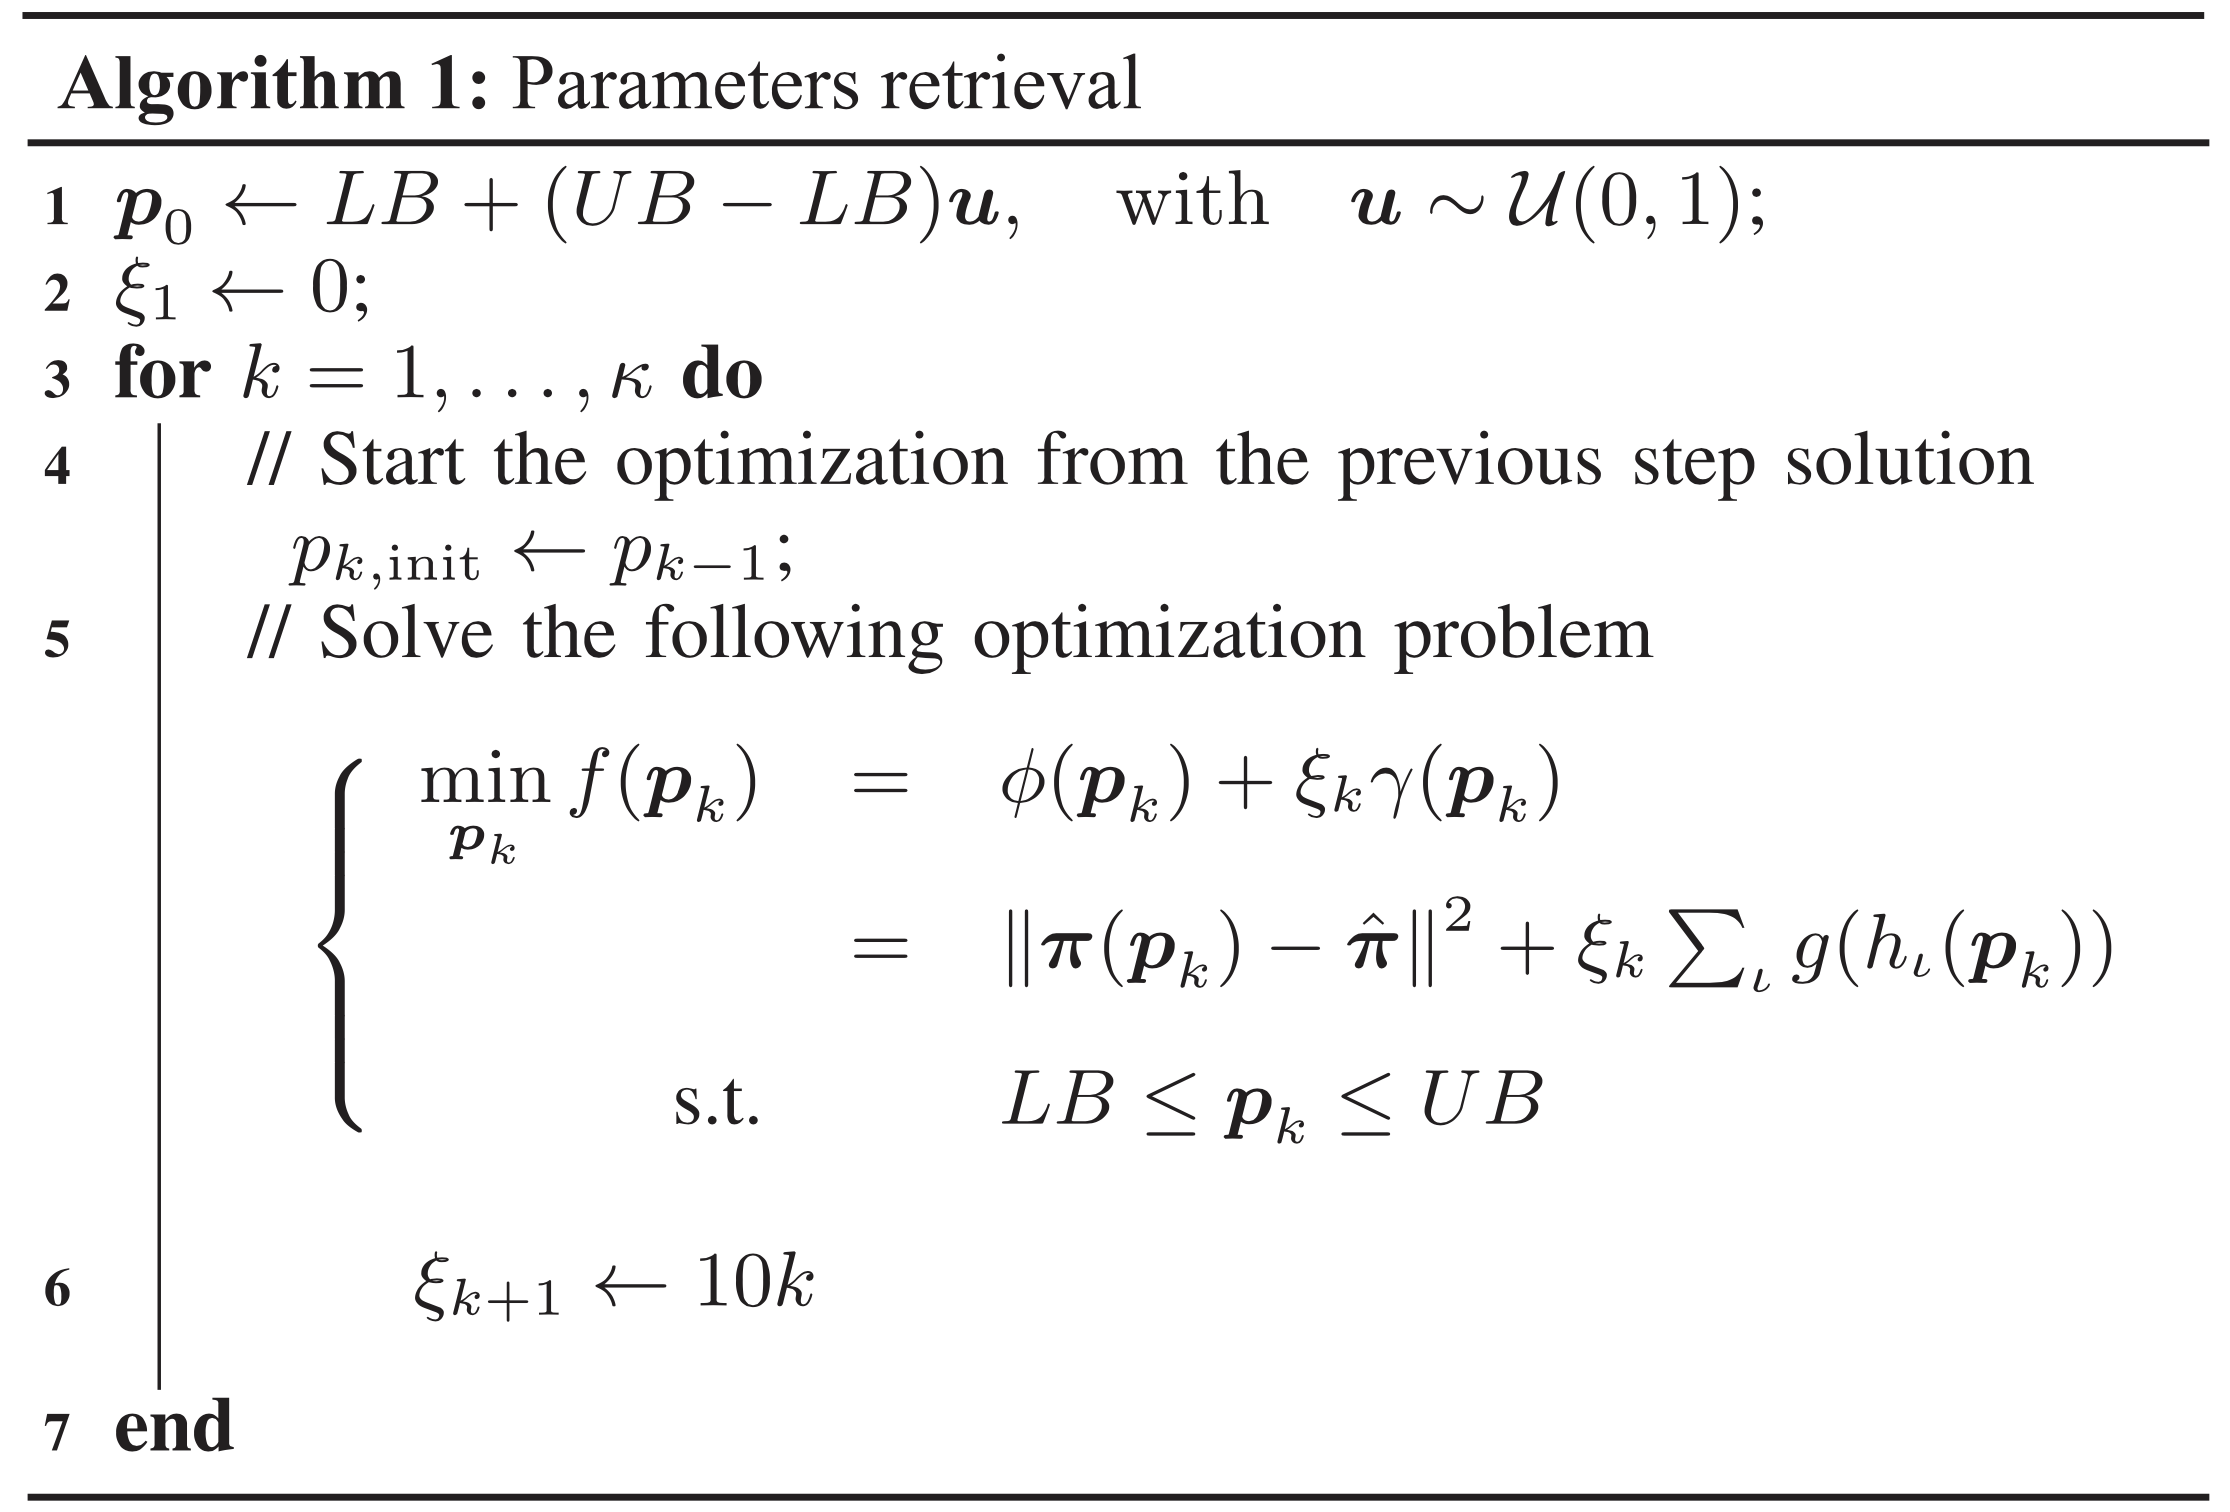
\includegraphics[width=0.6\textwidth]{images/3-dof/algorithm.png}
\caption{PBPR algorithm}
\end{figure}
\FloatBarrier
In particular, in addition to the lower and upper bounds, for each link $l_i$ the following triangle inequalities regarding the inertias must be satisfied:

\[\begin{cases}
\overline{I}_{i,x}+\overline{I}_{i,y} > \overline{I}_{i,z} \\
\overline{I}_{i,z}+\overline{I}_{i,y} > \overline{I}_{i,x} \\
\overline{I}_{i,x}+\overline{I}_{i,z} > \overline{I}_{i,y}
\end{cases}\]

\noindent These inequalities can be rewritten as:

\[\frac{tr(I_{l_i})}{2}-\lambda_{max}(I_{l_i})>0\]

\noindent Moreover, the total sum of the link masses must be in a given range, that is:

\[m_{rob,min}\le \sum_i{m_i} \le m_{rob,max}\]

The search algorithm is simulated annealing as before and we run the algorithm 3 times.

\subsection{Tree of solutions}
The tree algorithm is a simple extension of the 1R case; we highlight the fact that segments of different links are put together (so that we do not give priority to any link) and examined through the heuristic function based on the condition number. The algorithm used to solve the optimization problems of the tree is pattern search like in the previous case.
\\\\
After the tree has been built, we have the sequence of most likely signs that we apply to the absolute torques. Finally, we run the PBPR algorithm to the torques with the estimated signs for 3 times by using simulated annealing as search algorithm.

\subsection{Experiments}
\paragraph{}We remember that the starting configuration of the robot is $q_1 = 0$, $q_2 = -\pi/2$ and $q_3 = 0$. So, we have generated some trajectories starting from 0 (that we will use for the first and third link) and others starting from $-\pi/2$ (that we will use for the second link) with the generate\_exciting\_traj() function.

\paragraph{Experiment 1}
The first trajectory generated is:
\begin{figure}[!htbp]
\centering
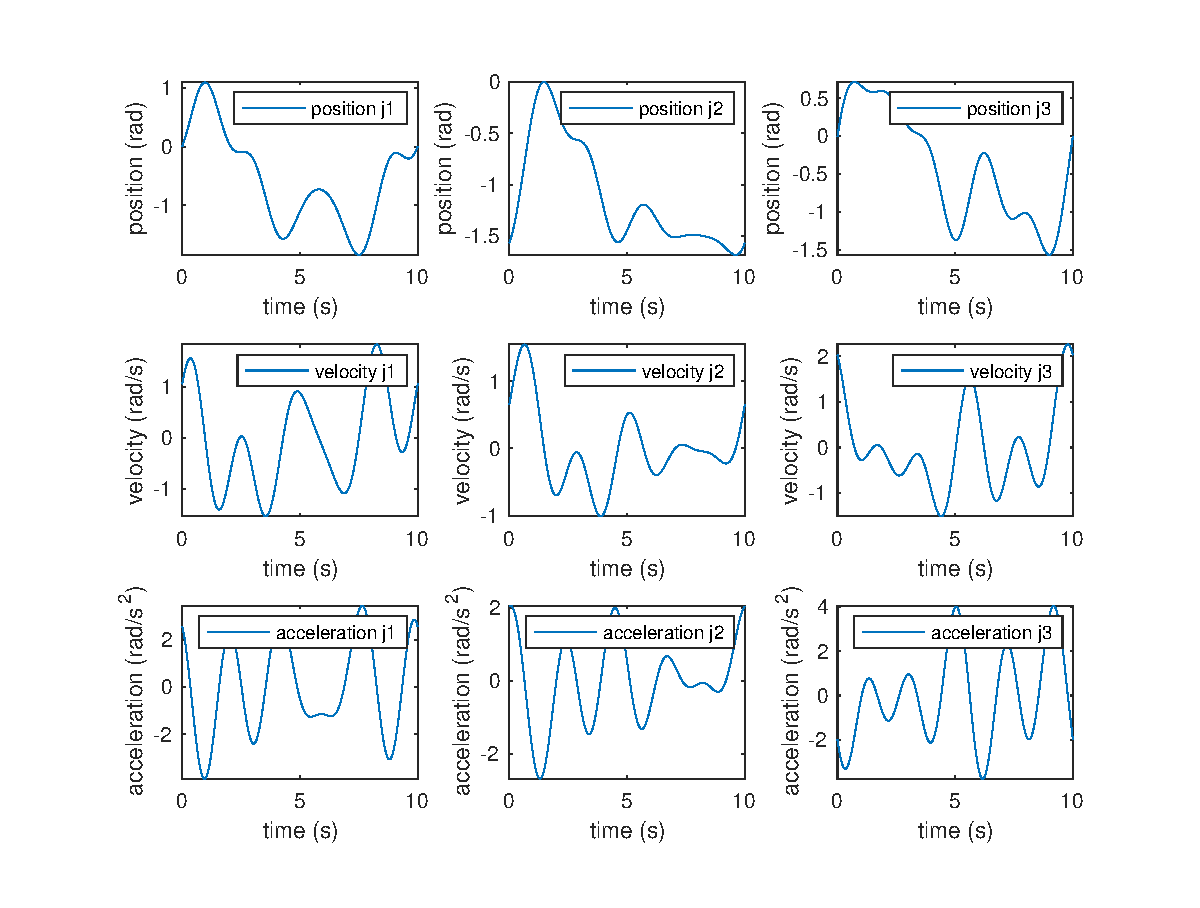
\includegraphics[width=0.7\textwidth]{images/3-dof/trajectory123.eps}
\caption{Plot of position, velocity and acceleration for each joint; the last two are obtained by symbolic differentiation}
\end{figure}
\FloatBarrier

From this data we generate torques and we send $\overline{Y}$ and $\overline{\tau}$ with the estimated signs to the PBPR algorithm. This is what we obtain:

\begin{table}[!htbp]
\centering
\begin{tabular}{|c|cc|}
\hline
& Ground truth & Retrieved\\ 
\hline
$m_1$ & 10.0000 & 11.0382\\
$m_2$ & 1.1250 & 2.9066\\
$m_3$ & 0.7500 & 0.3877\\
$r_{c1x}$ &  0 & 0\\
$r_{c1y}$ & -0.1500 & -0.1637\\
$r_{c1z}$ & 0 & 0\\
$r_{c2x}$ & -0.1500 & -0.2057\\
$r_{c2y}$ & 0 & 0\\
$r_{c2z}$ & -0.0600 & 0\\
$r_{c3x}$ & -0.1000 & -0.0046\\
$r_{c3y}$ & 0 & 0\\
$r_{c3z}$ & 0 & 0\\
$I_{1yy}$ & 0.0042 & 0\\
$I_{2xx}$ & $4.6879\cdot 10^{-4}$ & 0.0008\\
$I_{2yy}$ & 0.0087 & 0\\
$I_{2zz}$ & 0.0087 & 0.0150\\
$I_{3xx}$ & 3.1253$\cdot 10^{-4}$ & 0\\
$I_{3yy}$ & 0.0025 & 0\\
$I_{3zz}$ & 0.0025 & 0\\
\hline
\end{tabular}
\caption{Dynamic parameters}
\end{table}
\FloatBarrier

The estimated dynamic coefficients are:

\[\hat{\pi}_1 = 0.0275\]
\[\hat{\pi}_2  = 0.0599\]
\[\hat{\pi}_3 = 0.0148\]
\[\hat{\pi}_4 = 0.0227\]
\[\hat{\pi}_5 = 0.0905\]
\[\hat{\pi}_6 = 0.0148\]
\[\hat{\pi}_7 = 0.0351\]
\[\hat{\pi}_8 = 0.0068\]
\[\hat{\pi}_9 = 3.8295\]
\[\hat{\pi}_{10} = 0.7431\]

We do not obtain the exactly same values of the dynamic coefficients; the error we obtain is equal to 0.0594.

\begin{figure}[!htbp]
\centering
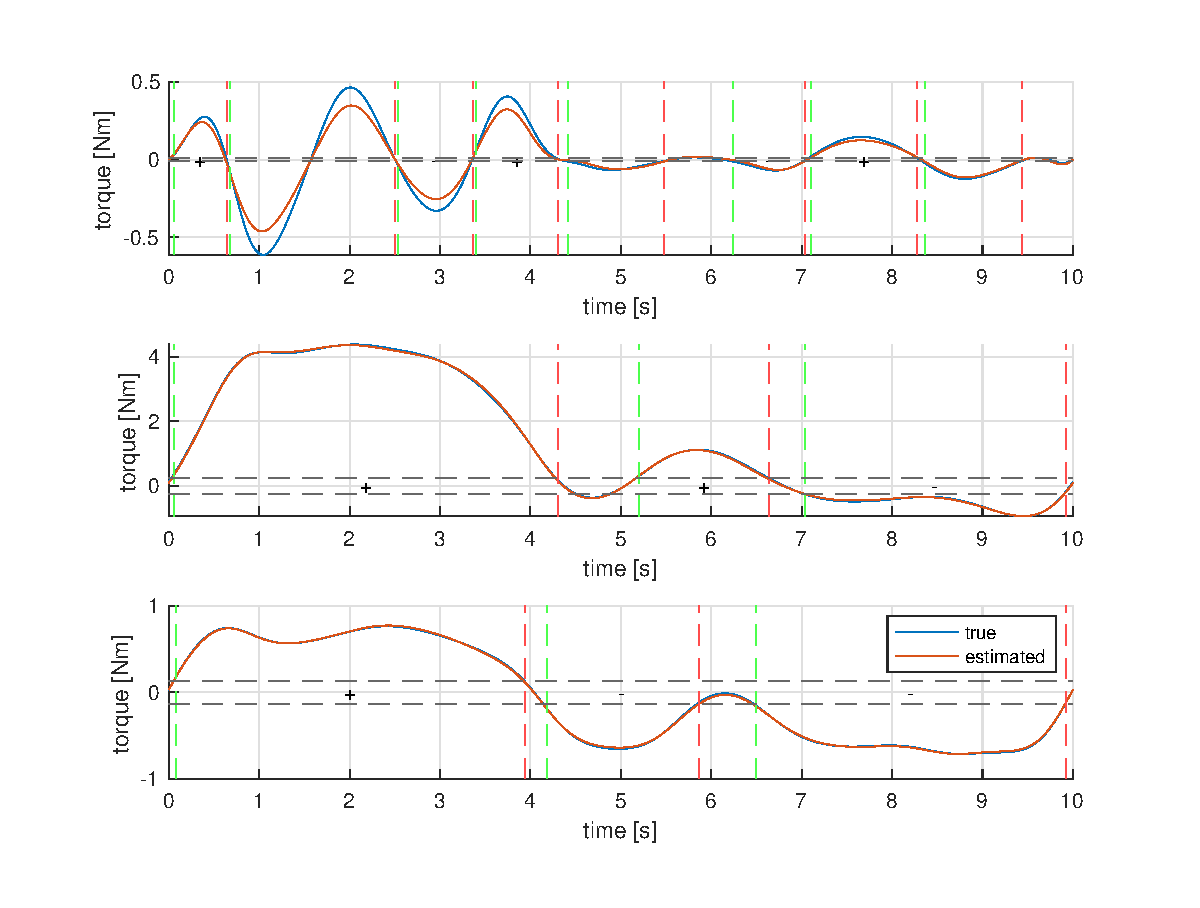
\includegraphics[width=0.7\textwidth]{images/3-dof/results1.eps}
\caption{Plot of the reconstructed torque vs nominal torque. The gray dashed lines represent the threshold; the green dashed lines represent the start of the segment, while the red dashed lines represent the end of the segment. Samples under threshold are discarded. The signs estimated by the algorithm are reported for each segment.}
\end{figure}
\FloatBarrier

As we can notice from the plot, the algorithm fails in predicting one sign in the first joint torque; this is why we have a discrepancy between the nominal torque and the reconstructed one. The reason of this error is because the algorithm has selected a threshold which was too low for the real problem, so it cannot recognize the change of sign in that particular section.

\paragraph{Experiment 2}
The second trajectory generated is:
\begin{figure}[!htbp]
\centering
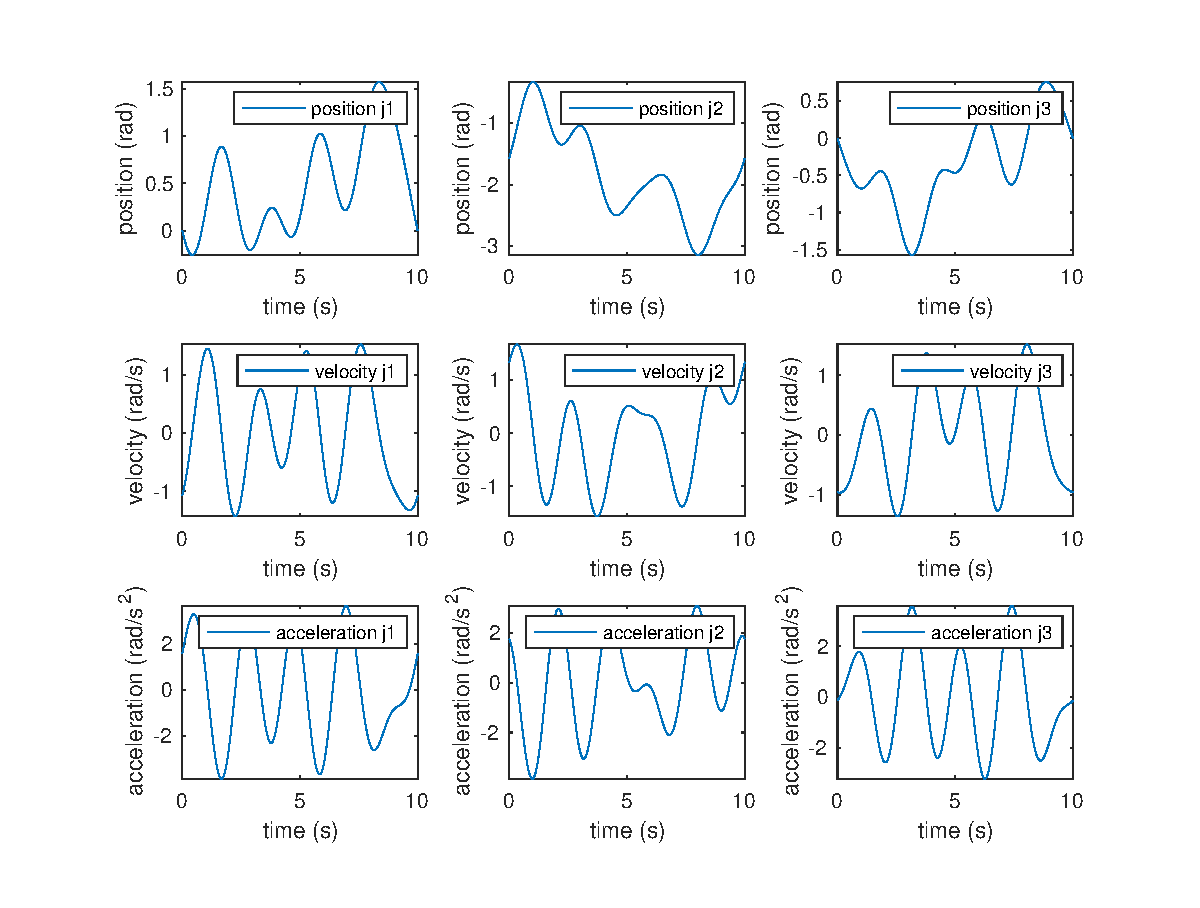
\includegraphics[width=0.7\textwidth]{images/3-dof/trajectory456.eps}
\caption{Plot of position, velocity and acceleration for each joint; the last two are obtained by symbolic differentiation}
\end{figure}
\FloatBarrier

From this data we do the same procedure as before. This is what we obtain:

\begin{table}[!htbp]
\centering
\begin{tabular}{|c|cc|}
\hline
& Ground truth & Retrieved\\ 
\hline
$m_1$ & 10.0000 & 11.0371\\
$m_2$ & 1.1250 & 1.0362\\
$m_3$ & 0.7500 & 0.6448\\
$r_{c1x}$ &  0 & 0\\
$r_{c1y}$ & -0.1500 & -0.1681\\
$r_{c1z}$ & 0 & 0\\
$r_{c2x}$ & -0.1500 & -0.1067\\
$r_{c2y}$ & 0 & 0\\
$r_{c2z}$ & -0.0600 & -0.0506\\
$r_{c3x}$ & -0.1000 & -0.0837\\
$r_{c3y}$ & 0 & 0\\
$r_{c3z}$ & 0 & 0\\
$I_{1yy}$ & 0.0042 & 0.0090\\
$I_{2xx}$ & $4.6879\cdot 10^{-4}$ & 0.0008\\
$I_{2yy}$ & 0.0087 & 0.0051\\
$I_{2zz}$ & 0.0087 & 0.0047\\
$I_{3xx}$ & 3.1253$\cdot 10^{-4}$ & 0.0008\\
$I_{3yy}$ & 0.0025 & 0.0019\\
$I_{3zz}$ & 0.0025 & 0.0014\\
\hline
\end{tabular}
\caption{Dynamic parameters}
\end{table}
\FloatBarrier

The estimated dynamic coefficients are:

\[\hat{\pi}_1 = 0.0363\]
\[\hat{\pi}_2  = 0.1010\]
\[\hat{\pi}_3 = 0.0099\]
\[\hat{\pi}_4 = 0.0225\]
\[\hat{\pi}_5 = 0.1116\]
\[\hat{\pi}_6 = 0.0102\]
\[\hat{\pi}_7 = 0.0456\]
\[\hat{\pi}_8 = 0.0068\]
\[\hat{\pi}_9 = 3.8627\]
\[\hat{\pi}_{10} = 0.7358\]

In this case, the dynamic coefficients retrieved are almost equal to the ground ones, in fact the error we obtain is equal to   $3.3696\cdot10^{-5}$ and is smaller than the previous experiment.

\begin{figure}[!htbp]
\centering
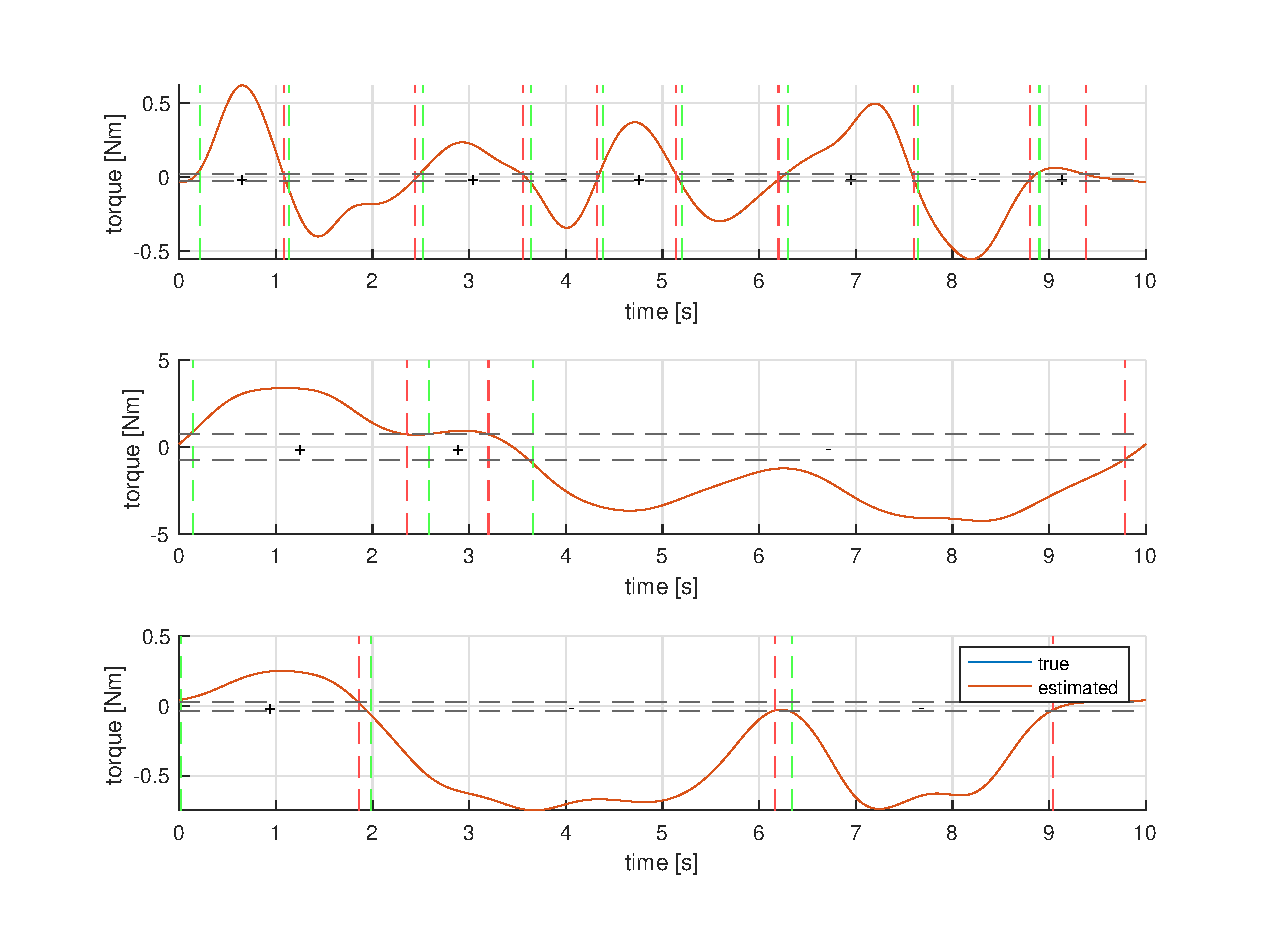
\includegraphics[width=0.7\textwidth]{images/3-dof/results2.eps}
\caption{Plot of the reconstructed torque vs nominal torque. The gray dashed lines represent the threshold; the green dashed lines represent the start of the segment, while the red dashed lines represent the end of the segment. Samples under threshold are discarded. The signs estimated by the algorithm are reported for each segment.}
\end{figure}
\FloatBarrier

From this figure we can see that the algorithm never fails in predicting torque signs; this is why the error is smaller than before and the torque reconstruction is better.

\subsection{Validation} \paragraph{} We validate the results obtained in the second experiment (because it is the one with the smaller error) on a new never seen trajectory:

\begin{figure}[!htbp]
\centering
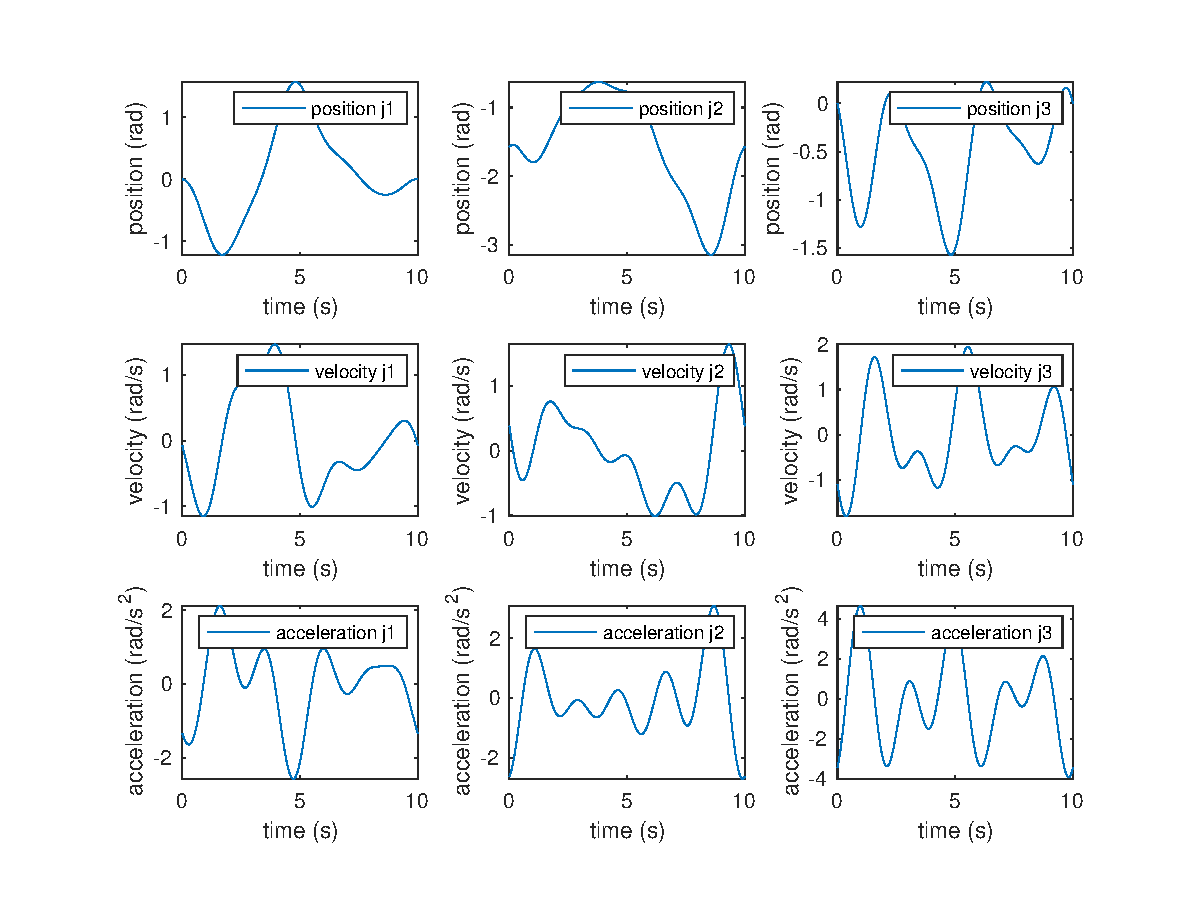
\includegraphics[width=0.7\textwidth]{images/3-dof/validation_trajectory.eps}
\caption{Plot of position, velocity and acceleration for each joint; the last two are obtained by symbolic differentiation}
\end{figure}
\FloatBarrier

The predicted torques are:

\begin{figure}[!htbp]
\centering
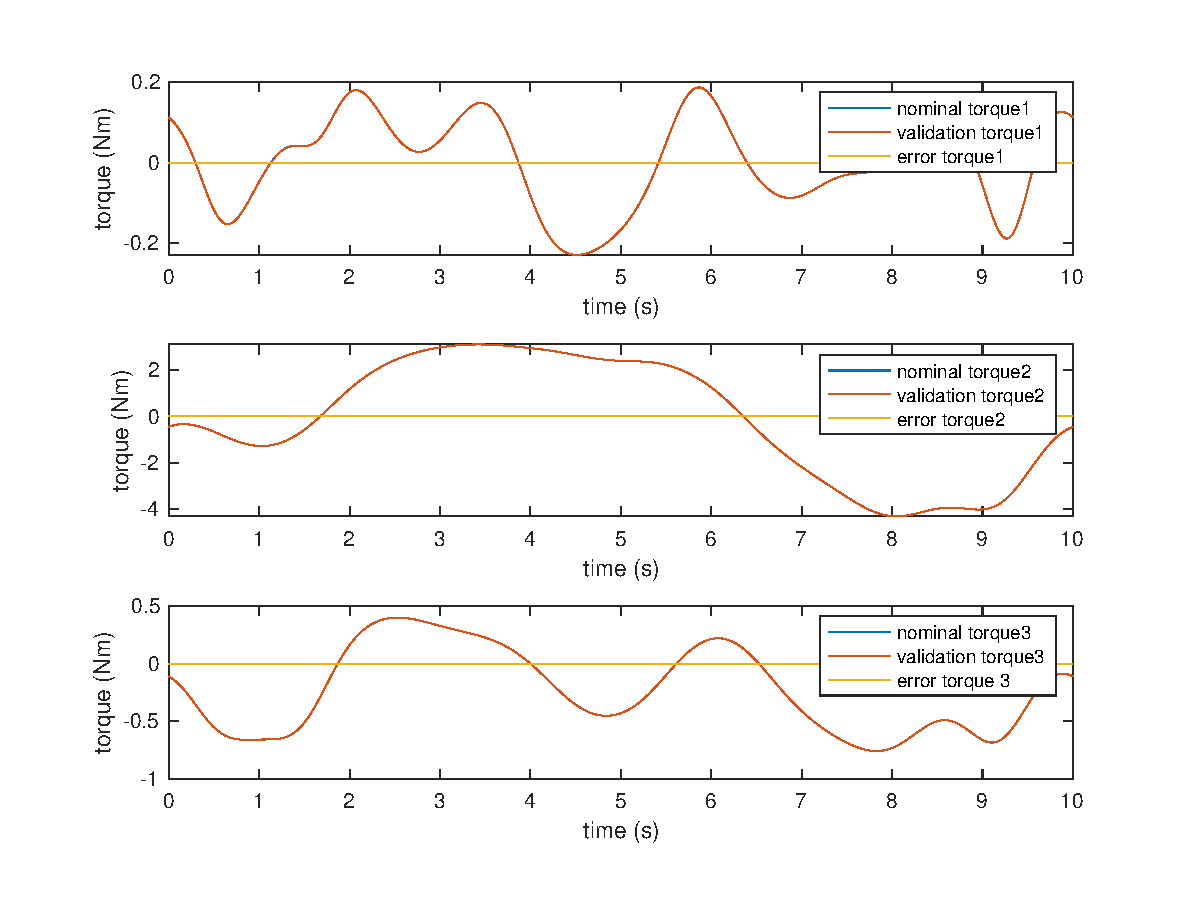
\includegraphics[width=0.7\textwidth]{images/3-dof/validation.eps}
\caption{Plot of the nominal torque vs validation torque for each link; the error is computed as nominal torque - validation torque}
\end{figure}
\FloatBarrier

\pagebreak
\section{7R robot: Franka Emika Panda}
At this stage we tried to apply our algorithm to a real robot: the Franka Emika Panda.\\
Choosing this particular robot we could re-use all data collected during the experimentation of the paper \emph{Dynamic Identification of the Franka Emika Panda Robot With Retrieval of Feasible Parameters Using Penalty-Based Optimization} (Gaz, Cognetti, Oliva, Giordano, De Luca). In fact in the paper repository (\href{https://github.com/marcocognetti/FrankaEmikaPandaDynModel}{\textcolor{red}{link to repo}}) there are stored some useful information used in the work, such as the regressor matrix $Y$ and the torque vector $\tau$.\\\\
As before, we proceeded by taking the absolute value of the torque, so to pretend that we didn't have this kind of information. At this stage we could apply our tree algorithm to estimate the signs.\\
By doing so, we faced a big problem: in fact, when the robot increases its complexity, the tree algorithm becomes tremendously slow and it takes days and weeks to finish its execution.\\\\
Being unable to use the algorithm as it is, we tried to relax some constraint while solving the optimization problems of the tree. By ignoring the constraints that ensure us physically consistent parameters we can re-write the optimization problem in the following form:
\[\begin{cases}\min_{p_k}{\phi(p_k)} = \lVert \overline{Y}\pi(p_k)-\overline{\tau} \rVert^2 + \xi_k \gamma(p_k)\\s.t. \qquad LB\le p_k \le UB\end{cases} \Rightarrow \quad min_{a}{\phi(a)} = \lVert \overline{Y}a-\overline{\tau} \rVert^2\]
But at this stage we know the solution in closed form, in fact it is the solution driven by the pseudoinverse of the regressor matrix
\[a^* = \overline{Y}^{\#}\overline{\tau}\]
Using this relaxed problem in the tree, and not checking for the physical meaning of each term, we end up with 2 best solutions: one the opposite of the other.
\[\overline{Y}a = \overline{\tau} \qquad \qquad and \qquad \qquad \overline{Y}(-a) = -\overline{\tau}\]
Of course only one of the two is physically consistent, and we don't know \emph{a priori} which is of the two. We can choose our final solution by running two times the PBPR algorithm and by checking the loss.\\\\
The fact that we do not take into account the physical constraints during the sign estimation, but we only check them at the end, leads to an incredible speed-up in the algorithm that is now able to estimate the two best possibilities for the torque signs in a time in the order of minutes.
In the following plot the results of this modified algorithm on the Franka Emika Panda are reported.
\FloatBarrier
\begin{figure}
\centering
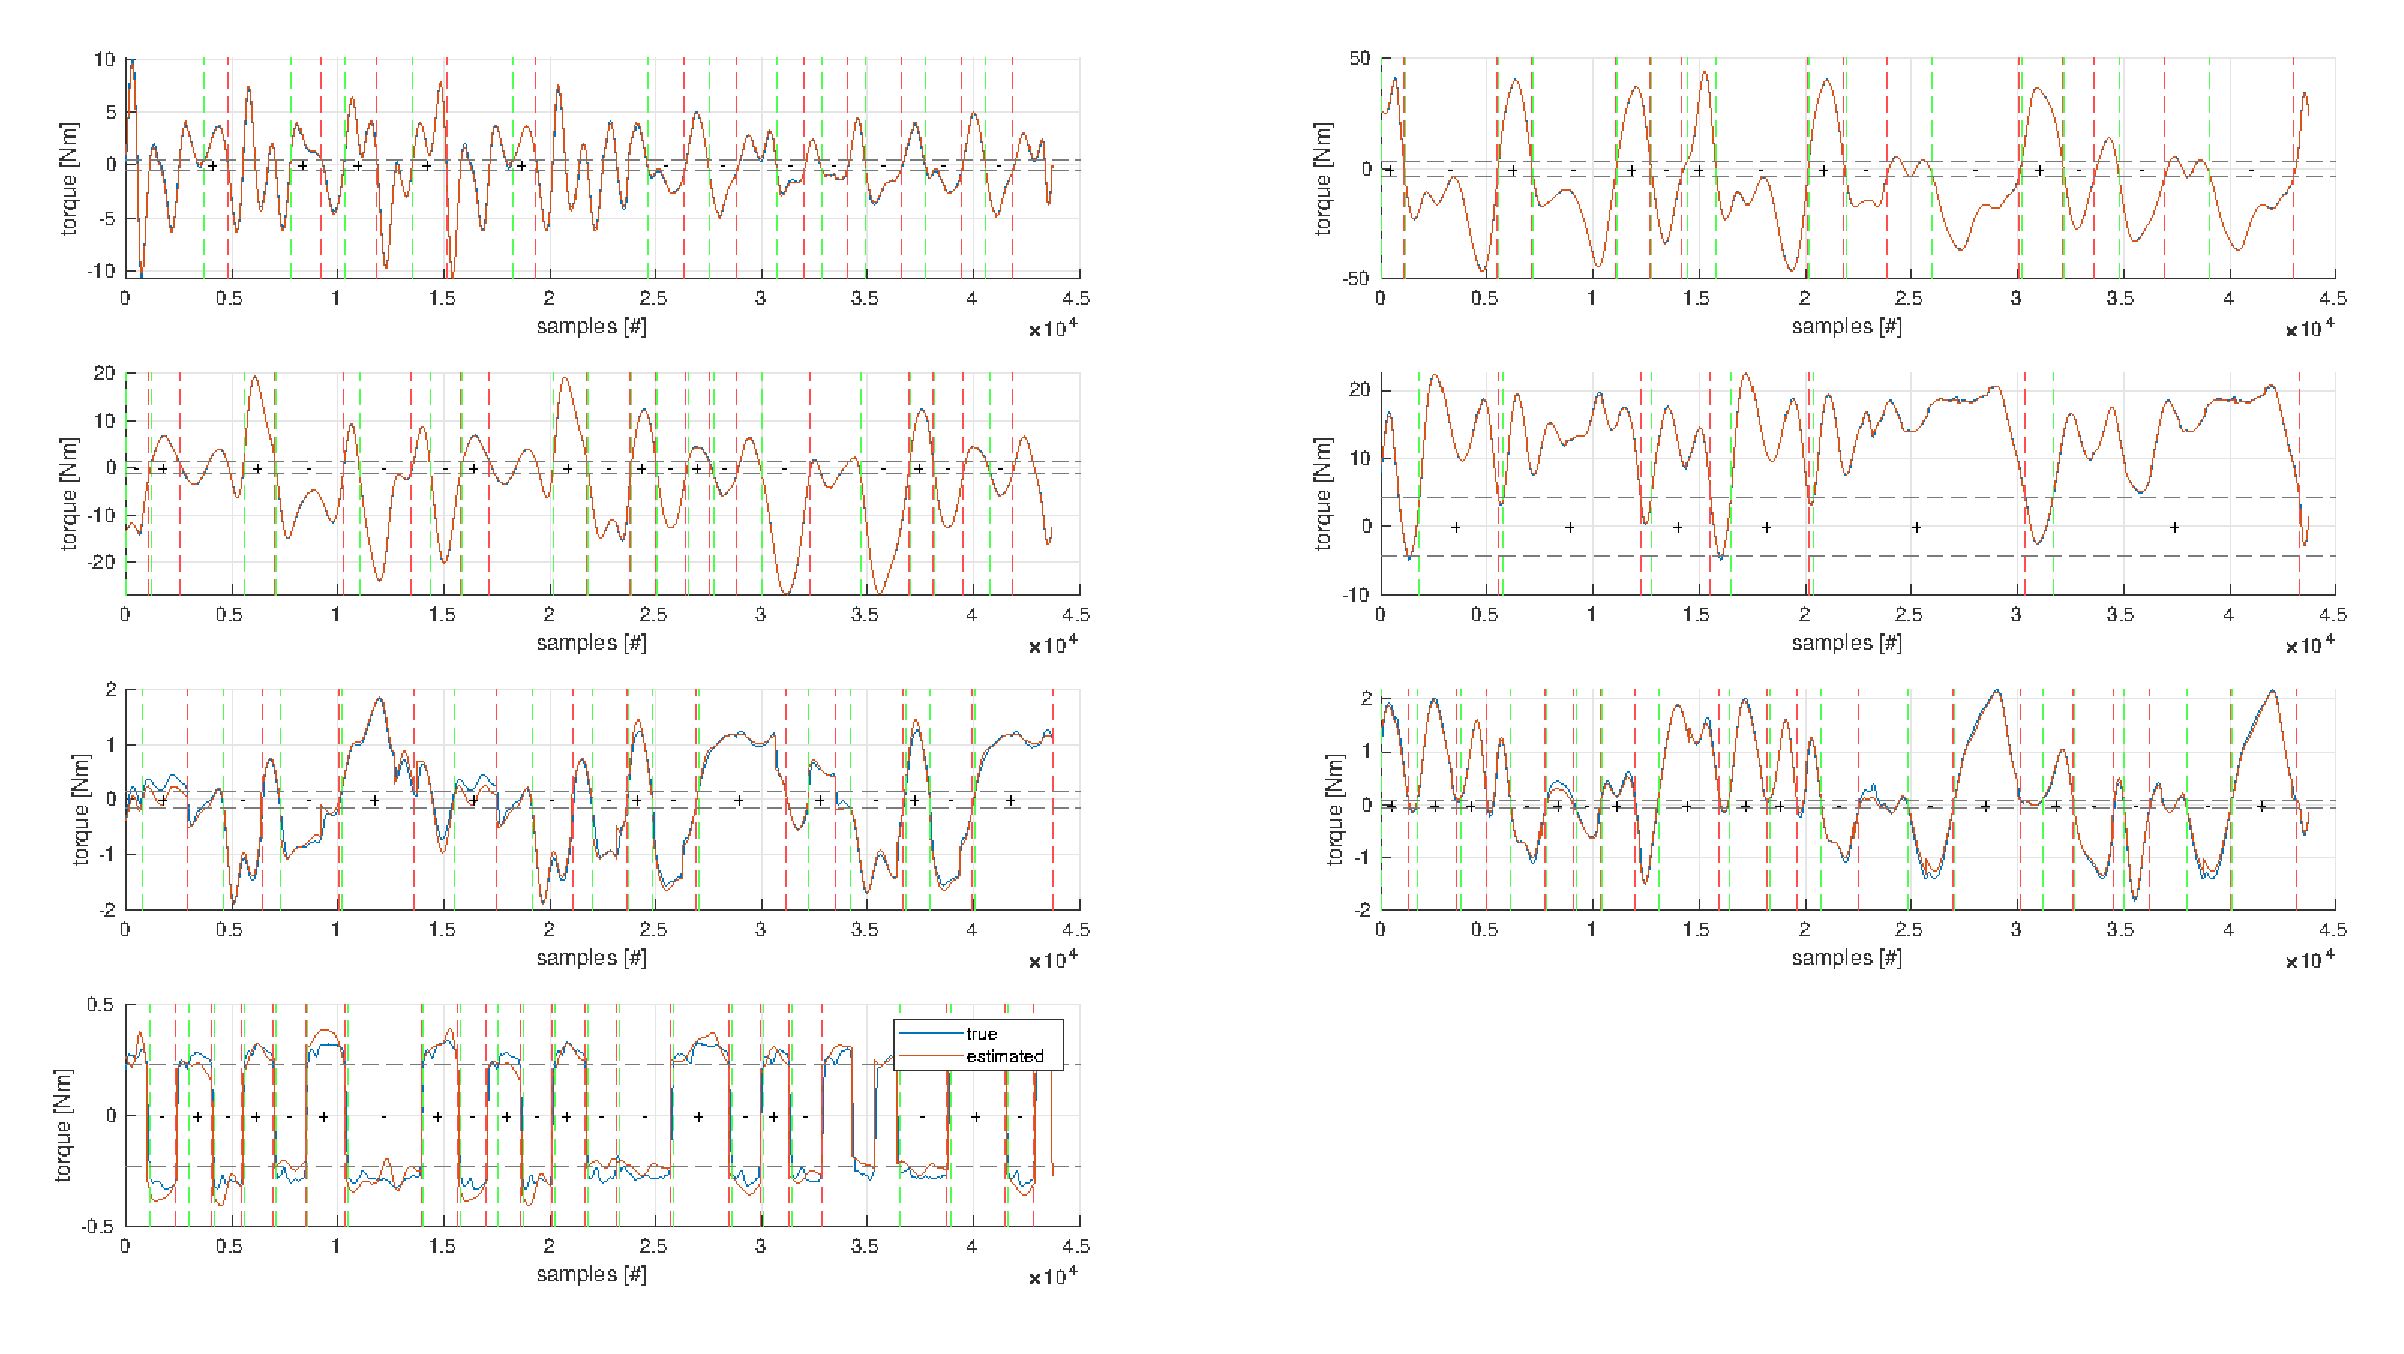
\includegraphics[width=1\textwidth]{images/franka_result_crop.eps}
\caption{Plot of the reconstructed torque vs nominal torque. The gray dashed lines represent the threshold; the green dashed lines represent the start of the segment, while the red dashed lines represent the end of the segment. Samples under threshold are discarded. The signs estimated by the algorithm are reported for each segment.}
\end{figure}
\FloatBarrier

We can see that the algorithm has been able to correctly identify 105 segment signs out of 105.\\
The norm of the difference between the retrieved coefficients and the ones estimated with the classical approach (if one has the sign information) is 0.3980.

\section{V-REP}
In this section we show the V-REP scenes for our two robots.

\subsection{1R arm}We have implemented a scene in V-REP from scratch, by taking a fixed base, a revolute joint and a link. We control the joint in position with the PID controller built in the joint. The arm is in 0 position at rest. The link is a parallelepiped which length is 1 $m$ and its transversal section is a square with side equal to 0.1 $m$. The mass of the link is 5 $kg$ and the principal moment of inertia is 0.4208 $kg\cdot m^2$. Since the arm has a uniform density, the center of mass is located at the center of the link, so it is 0.5 $m$ from the top.

\begin{figure}[!htbp]
\centering
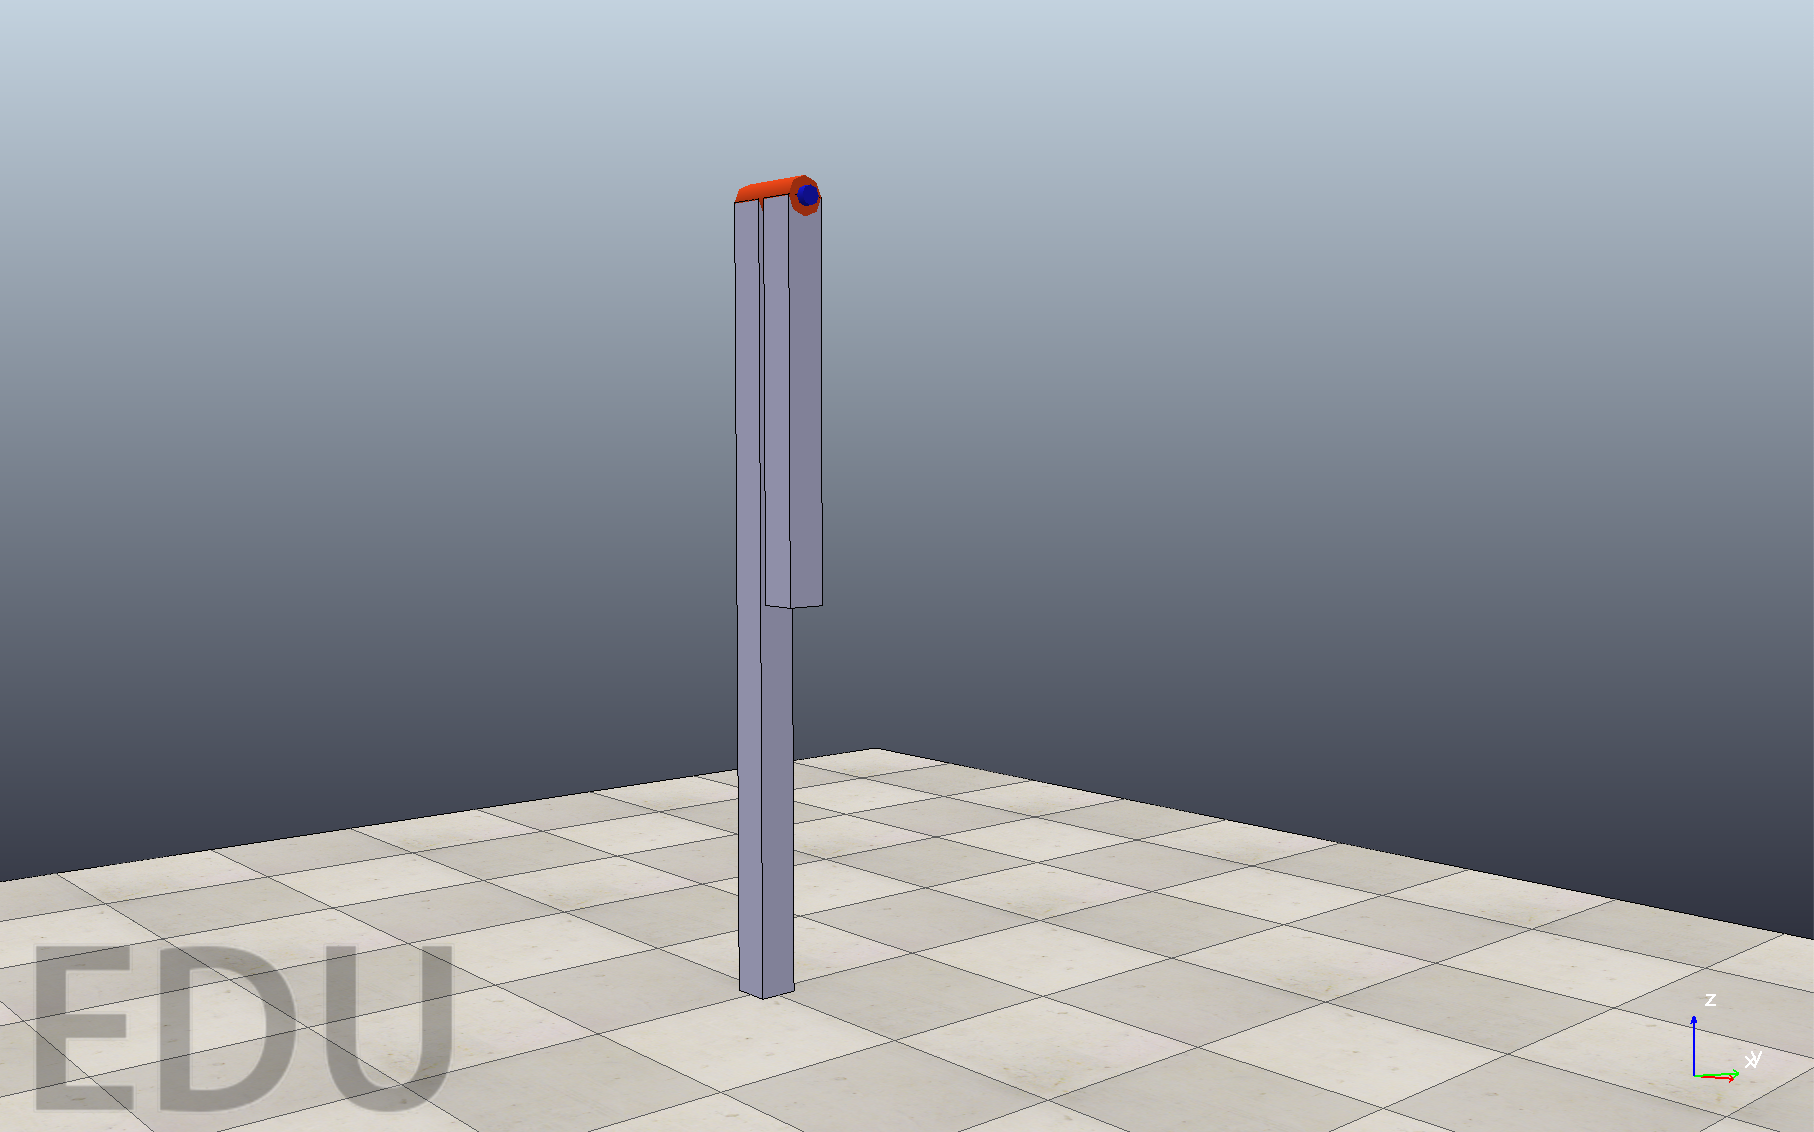
\includegraphics[width=0.7\textwidth]{images/1-dof/scene.png}
\caption{V-REP scene of the 1-dof robot arm}
\end{figure}
\FloatBarrier

\subsection{3R spatial arm} We created a new V-REP scene from scratch:
\FloatBarrier
\begin{figure}[!htbp]
\centering
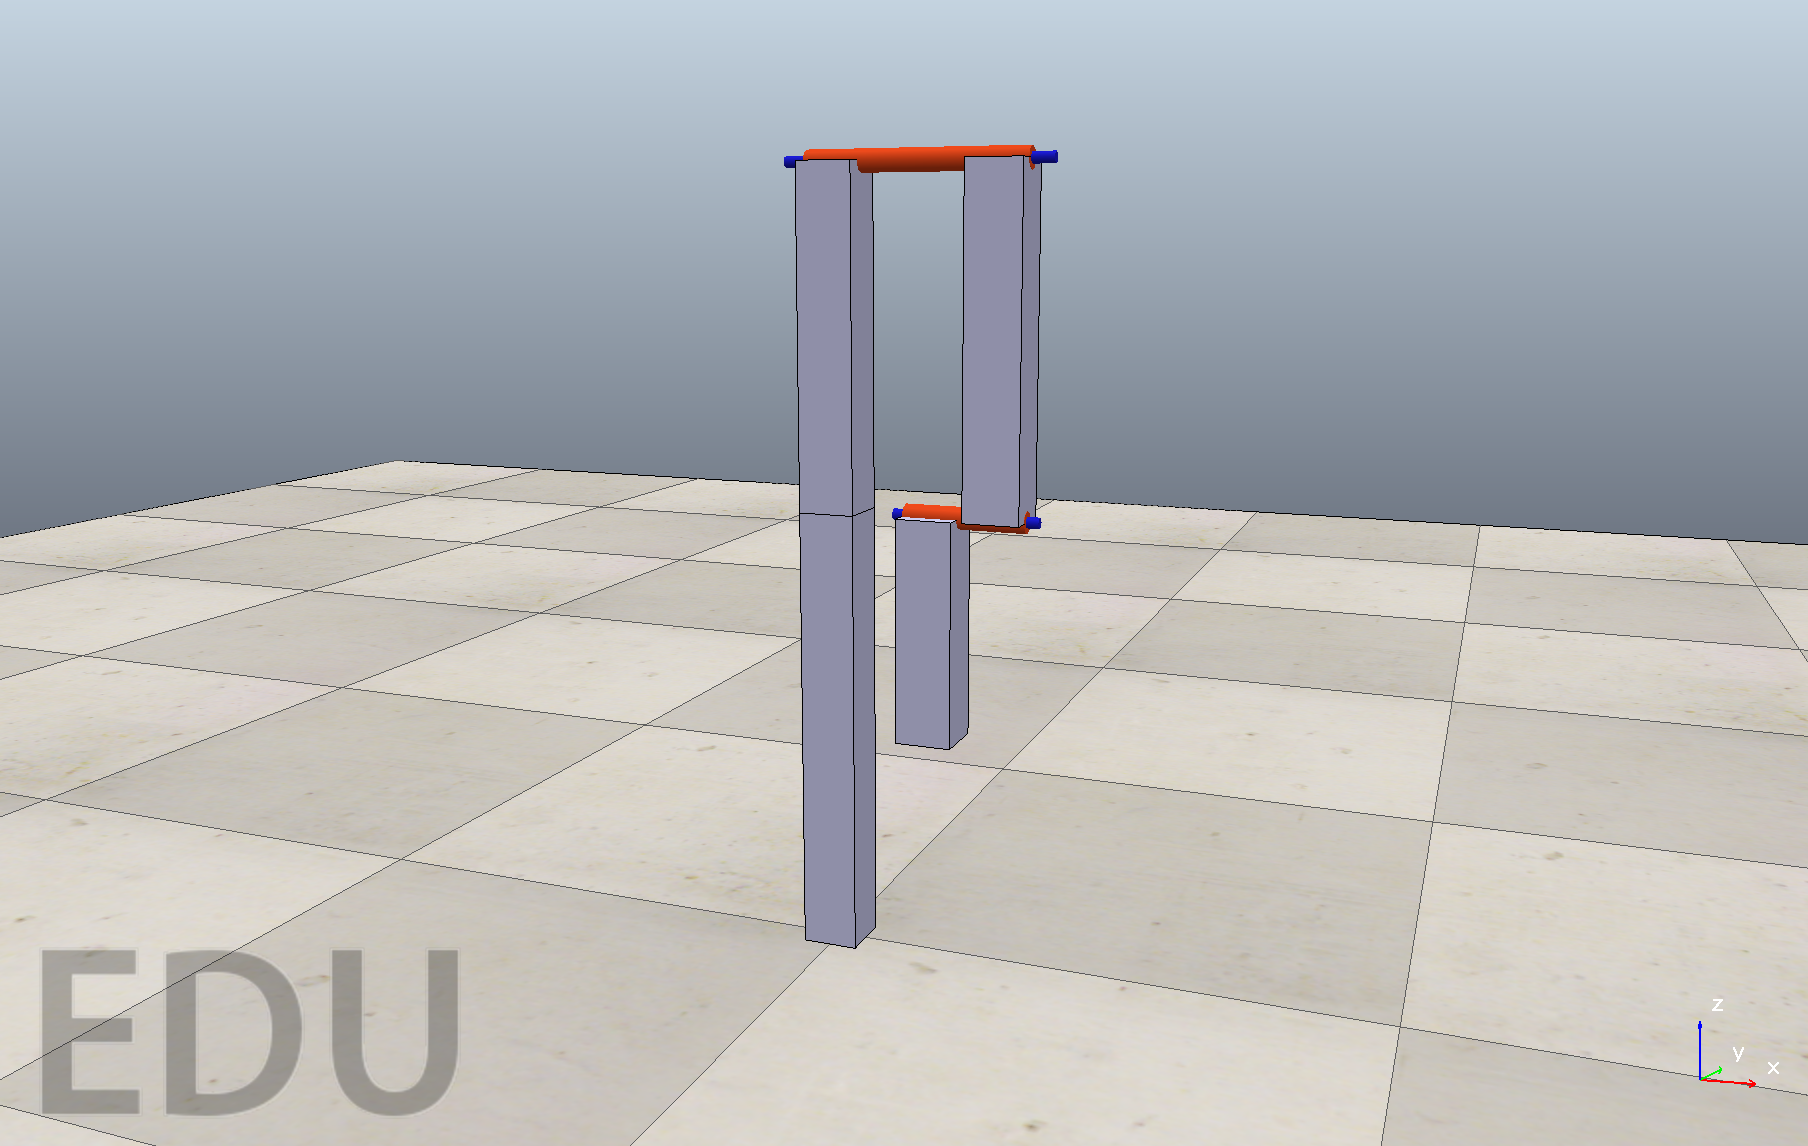
\includegraphics[width=0.7\textwidth]{images/3-dof/scene.png}
\caption{3R Robot-arm V-REP scene}
\end{figure}
\FloatBarrier

The first and the second links are two parallelepipeds whose length is 0.3 $m$ and their transversal section is a square with side equal to 0.05 $m$, while the third link is 0.2 $m$ long and has a transversal section that is a square with side equal to 0.05 $m$.

We report the  values for masses and inertia tensors.
\[m_1 = 10 \;kg,\quad I_{xx,1} = 7.708\cdot 10^{-2}\;kg\cdot m^2,\quad I_{yy,1} = 4.167 \cdot 10^{-3}\;kg\cdot m^2,\quad I_{zz,1} = 7.708\cdot 10^{-2}\;kg\cdot m^2\]
\[ m_2 = 1.125\;kg,\quad I_{xx,2} = 4.6879\cdot10^{-4}\;kg\cdot m^2,\quad I_{yy,2} = 8.6715\cdot 10^{-3}\;kg\cdot m^2,\quad I_{zz,2} = 8.6715\cdot 10^{-3}\;kg\cdot m^2\]
\[m_3 = 0.75\;kg,\quad I_{xx,3} = 3.1252\cdot 10^{-4}\;kg\cdot m^2,\quad I_{yy,3} = 2.6565\cdot 10^{-3}\;kg\cdot m^2,\quad I_{zz,3} = 2.6565\cdot 10^{-3}\;kg\cdot m^2\]

\section{Conclusions}
From the results obtained, we can state that the algorithm proposed for torque sign estimation works well. In fact, whenever we have a segment predicted well (that is, in which the sign does not change), the algorithm guess the right  sign. The problem is when the threshold is not identified correctly, but this seldom happens. \\\\

However, we can idenitfy two drawbacks of the proposed algorithm: the first one regards the fact that we discard under-threshold samples (which are at least 10\% of the total); moreover, too short segments are discarded too. The second drawback is that the algorithm becomes slower and slower as the robot complexity increases.
\clearpage

\begin{thebibliography}{}
\bibitem{1}
C. Gaz, M. Cognetti, A. Oliva, P. R. Giordano, A. De Luca
\emph {Dynamic Identification of the Franka Emika Panda Robot With Retrieval of Feasible Parameters Using Penalty-Based Optimization}
\bibitem{2}
C. Gaz, M. Cognetti, A. Oliva, P. R. Giordano, A. De Luca
\emph {Dynamic Identification of the Franka Emika Panda Robot With Retrieval of Feasible Parameters Using Penalty-Based Optimization – Supplementary material (revised version: October $15^{th}$, 2019)}
\bibitem{3}
A. De Luca
\emph {Slides of the Robotics I/II courses}
\end{thebibliography}

\end{document}